\documentclass[11pt, a4paper]{article}
\usepackage[a4paper, margin=2.3cm]{geometry}
\usepackage[utf8]{inputenc}
\usepackage[T1]{fontenc}
\usepackage[english]{babel}
\usepackage{lmodern}
\renewcommand{\familydefault}{\sfdefault}

\usepackage{amsmath, amssymb, amsthm}
\usepackage{mathtools}
\usepackage{booktabs}
\usepackage{array}
\usepackage{enumitem}
\usepackage{xcolor}
\usepackage{tcolorbox}
\tcbuselibrary{breakable}
\usepackage{tikz}
\usetikzlibrary{arrows.meta, calc}
\usepackage{pgfplots}
\pgfplotsset{compat=1.18}
\usepackage[colorlinks=true, linkcolor=navy, citecolor=navy, urlcolor=navy]{hyperref}

% Palette
\definecolor{navy}{RGB}{22, 58, 108}
\definecolor{intuitionbg}{RGB}{236, 244, 253}
\definecolor{intuitionframe}{RGB}{32, 96, 172}
\definecolor{thmbg}{RGB}{247, 248, 250}
\definecolor{thmframe}{RGB}{70, 88, 112}
\definecolor{accentred}{RGB}{180, 42, 42}
\definecolor{accentteal}{RGB}{18, 122, 114}

% Theorem environments (amsthm + tcolorbox framing)
\theoremstyle{definition}
\newtheorem{definition}{Definition}[section]
\newtheorem{example}[definition]{Example}
\newtheorem{algorithm}[definition]{Algorithm}

\theoremstyle{plain}
\newtheorem{theorem}[definition]{Theorem}
\newtheorem{proposition}[definition]{Proposition}
\newtheorem{lemma}[definition]{Lemma}
\newtheorem{corollary}[definition]{Corollary}

\tcolorboxenvironment{definition}{
  breakable, colback=thmbg, colframe=thmframe,
  boxrule=0.6pt, arc=2pt, left=7pt, right=7pt, top=5pt, bottom=5pt
}
\tcolorboxenvironment{proposition}{
  breakable, colback=thmbg, colframe=navy,
  boxrule=0.7pt, arc=2pt, left=7pt, right=7pt, top=5pt, bottom=5pt
}
\tcolorboxenvironment{theorem}{
  breakable, colback=thmbg, colframe=navy,
  boxrule=0.8pt, arc=2pt, left=7pt, right=7pt, top=5pt, bottom=5pt
}
\tcolorboxenvironment{lemma}{
  breakable, colback=thmbg, colframe=thmframe,
  boxrule=0.6pt, arc=2pt, left=7pt, right=7pt, top=5pt, bottom=5pt
}
\tcolorboxenvironment{corollary}{
  breakable, colback=thmbg, colframe=thmframe,
  boxrule=0.6pt, arc=2pt, left=7pt, right=7pt, top=5pt, bottom=5pt
}
\tcolorboxenvironment{example}{
  breakable, colback=white, colframe=thmframe!65,
  boxrule=0.5pt, arc=2pt, left=7pt, right=7pt, top=5pt, bottom=5pt
}
\tcolorboxenvironment{algorithm}{
  breakable, colback=thmbg, colframe=accentteal,
  boxrule=0.7pt, arc=2pt, left=7pt, right=7pt, top=5pt, bottom=5pt
}

% Custom blue Intuition box
\newtcolorbox{intuition}[1][Intuition]{
  breakable,
  colback=intuitionbg,
  colframe=intuitionframe,
  fonttitle=\bfseries,
  title={#1},
  boxrule=0.75pt,
  arc=2pt,
  left=8pt,
  right=8pt,
  top=5pt,
  bottom=5pt
}

\title{\textbf{Agile and Legged Robots (Module I)}\\[4pt]
\Large Dynamic Models and How to Read Them}
\author{Based on lectures by Leonardo Lanari}
\date{}

\begin{document}
\maketitle
\tableofcontents
\bigskip

% ============================================================================
\section{Overview, Five Small Systems, and Conventions \emph{(slides 1--7)}}
% ============================================================================

\subsection{Why Dynamic Models and Why Five Small Systems? \emph{(slides 2--4)}}

Counting degrees of freedom $m$ and independent control inputs $p$ tells us whether a robot is \emph{underactuated} ($p < m$), but counting alone cannot predict how the robot moves, where it can rest, or how fast it falls. Answering those questions requires a dynamic model.

Although software packages compute the dynamic matrices of an arbitrary multi-body robot in microseconds, deriving a small set of canonical models by hand is indispensable. Subsequent control chapters rely not on the raw numerical entries of the matrices, but on their \emph{structural properties}:
\begin{itemize}
  \item which equation contains no control input;
  \item which coordinate the mechanical energy does not depend on;
  \item where an inertial coupling term vanishes or changes sign.
\end{itemize}

\begin{intuition}
A derivation ends with a boxed matrix equation. That is \emph{not} the end of the story---it is where the study of the model begins. Only two full derivations are needed (the cart--pendulum and the two-link pendulum); the remaining systems are either special cases or take three lines to derive.
\end{intuition}

All five systems studied in this lecture use \emph{minimal coordinates} ($n = m$, so the coordinates are independent and unconstrained). Legged robots such as the compass walker and floating-base models are deferred because they involve unilateral contact forces and impacts.

\begin{table}[ht]
\centering
\caption{The five canonical systems covered in this lecture \emph{(slide 3)}.}
\label{tab:five_systems}
\renewcommand{\arraystretch}{1.2}
\begin{tabular}{@{}l c c p{8.4cm}@{}}
\toprule
\textbf{System} & $m$ & $p$ & \textbf{Why it is studied} \\
\midrule
Pendulum & $1$ & $1$ or $0$ & The building block: every other model reduces to it in some limit. \\
Cart--pendulum & $2$ & $1$ & A passive joint moved by the acceleration of its support. \\
Two-link pendulum (Acrobot, Pendubot) & $2$ & $1$ & A passive joint moved by inertial coupling; one mechanism, two placements of the motor. \\
Reaction-wheel pendulum & $2$ & $1$ & A passive body moved by an internal reaction torque. \\
Planar VTOL & $3$ & $2$ & No inertial coupling: a force whose direction is fixed in the body. \\
\bottomrule
\end{tabular}
\end{table}

\subsection{Five Questions for Every Model \emph{(slide 5)}}

To read every model systematically, we ask the same five questions (Q1--Q5) of each system. Table~\ref{tab:five_questions} links each question to its analytical tool and the downstream control chapters where it is used.

\begin{table}[ht]
\centering
\caption{The five structural questions asked of every dynamic model \emph{(slide 5)}.}
\label{tab:five_questions}
\renewcommand{\arraystretch}{1.2}
\begin{tabular}{@{}l p{6.8cm} p{3.6cm} l@{}}
\toprule
\textbf{ID} & \textbf{Question} & \textbf{Tool} & \textbf{Used in} \\
\midrule
\textbf{Q1} & \emph{Structure.} Which equations contain an input? What do the others say? & Reading $M, h, G, B$ & Ch.~4 \\
\textbf{Q2} & \emph{Conserved quantities.} Is energy conserved? Is a momentum conserved? & Power balance, cyclic coordinates & Ch.~6, 9 \\
\textbf{Q3} & \emph{Equilibria.} Where can the system rest, without input and with a constant input? & $G(q_e) = B(q_e)u_e$ & Ch.~4, 7 \\
\textbf{Q4} & \emph{Small motions.} Near an equilibrium, does it oscillate or fall? How fast? & Linearization & Ch.~5, 7 \\
\textbf{Q5} & \emph{Coupling.} Through which term does the input reach coordinates without a motor? Where does it vanish? & Off-diagonal inertia $M_{ij}$ or $B(q)$ & Ch.~4, 8 \\
\bottomrule
\end{tabular}
\end{table}

\noindent\emph{Roadmap to later chapters:} Ch.~4 covers control problems and the passive equation; Ch.~5 controllability; Ch.~6 integrability; Ch.~7 stabilization of equilibria; Ch.~8 zero dynamics; Ch.~9 energy and swing-up.

\subsection{Conventions and Reference Parameter Values \emph{(slides 6--7)}}

Throughout the lecture we adopt a fixed geometric convention:
\begin{itemize}
  \item Right-handed inertial frame $(x, y, z)$: $x$ horizontally to the right, $z$ vertically upward, $y$ pointing out of the page.
  \item Planar mechanisms move in the $x$--$z$ plane ($y=0$); gravity acts along $-z$ with $g = 9.81\,\mathrm{m/s^2}$.
  \item Angles are measured from the \emph{downward} vertical, positive counterclockwise. \textbf{Exception:} for the cart--pendulum, the pole angle $\theta$ is measured from the \emph{upward} vertical, positive clockwise.
  \item Because $e_x \times e_z = -e_y$, a counterclockwise angular rate $\dot{\theta}$ in the $x$--$z$ drawing corresponds to the 3D angular velocity vector $\omega = -\dot{\theta}\, e_y$.
  \item Because $m$ denotes the number of degrees of freedom, physical masses carry subscripts or capital letters ($m_p, m_1, m_v, M$).
\end{itemize}

\begin{table}[ht]
\centering
\caption{Reference physical parameters used for all numerical examples \emph{(slide 7)}.}
\label{tab:ref_values}
\renewcommand{\arraystretch}{1.2}
\begin{tabular}{@{}l p{6.8cm} p{4.6cm}@{}}
\toprule
\textbf{System} & \textbf{Reference values} & \textbf{Derived quantities} \\
\midrule
Pendulum & Point mass $m_p = 0.5\,\mathrm{kg}$ at $\ell_c = 0.4\,\mathrm{m}$ & $I_h = 0.08\,\mathrm{kg\,m^2}$, $m_p g \ell_c = 1.96\,\mathrm{Nm}$ \\
Cart--pendulum & Cart $M = 1\,\mathrm{kg}$; uniform rod pole $m_p = 0.2\,\mathrm{kg}$, length $0.6\,\mathrm{m}$ & $\ell_c = 0.3\,\mathrm{m}$, $I_h = 0.024\,\mathrm{kg\,m^2}$ \\
Two-link pendulum & Uniform rods: $m_1 = 1\,\mathrm{kg}$, $\ell_1 = 0.3\,\mathrm{m}$; $m_2 = 0.5\,\mathrm{kg}$, $\ell_2 = 0.3\,\mathrm{m}$ & $\ell_{ci} = \ell_i/2$, $I_i = m_i \ell_i^2 / 12$ \\
Reaction wheel & $I_b = 0.04\,\mathrm{kg\,m^2}$, $I_w = 0.001\,\mathrm{kg\,m^2}$, $\kappa = 1.5\,\mathrm{Nm}$ & --- \\
\bottomrule
\end{tabular}
\end{table}

% ============================================================================
\section{Part 1: The Method \emph{(slides 8--23)}}
% ============================================================================

\subsection{Energies, Positions, and Velocities \emph{(slides 9--10)}}

Consider a mechanism of rigid links described by independent generalized coordinates $q \in \mathbb{R}^m$. For link $i$, let $r_{ci}(q) \in \mathbb{R}^3$ be the position of its center of mass (CoM), $\omega_i \in \mathbb{R}^3$ its angular velocity, and $I_{ci}$ its inertia tensor about the CoM (expressed in the same frame as $\omega_i$).

\begin{definition}[Kinetic Energy, Potential Energy, and Lagrangian]
The total kinetic energy $T$, gravitational potential energy $V$, and Lagrangian $L$ of a rigid-body mechanism are
\[
  T = \sum_{i} \left( \frac{1}{2} m_i \|\dot{r}_{ci}\|^2 + \frac{1}{2} \omega_i^T I_{ci} \omega_i \right), \qquad
  V = \sum_{i} m_i g z_{ci}, \qquad
  L(q, \dot{q}) = T(q, \dot{q}) - V(q).
\]
In planar motion ($r_{ci} = (x_{ci}, 0, z_{ci})^T$), each link rotates about the normal to the $x$--$z$ plane with scalar rate $\omega_i$ and scalar CoM inertia $I_i$, simplifying the kinetic energy to
\[
  T = \sum_{i} \left( \frac{1}{2} m_i \|\dot{r}_{ci}\|^2 + \frac{1}{2} I_i \omega_i^2 \right).
\]
\end{definition}

\begin{intuition}
A common pitfall is confusing $\omega_i$ with the angular velocity of the position vector $r_{ci}$. Remember: $\omega_i$ is the rotation rate of the \emph{rigid link itself}. If a link translates along a circular path without turning (like a Ferris wheel cabin), its CoM moves ($\dot{r}_{ci} \neq 0$) while its orientation is fixed ($\omega_i = 0$), so $T_i = \frac{1}{2} m_i \|\dot{r}_{ci}\|^2$. Conversely, a balanced wheel spinning on a fixed axle has $\dot{r}_{ci} = 0$ and $T_i = \frac{1}{2} I_i \omega_i^2$.
\end{intuition}

\begin{figure}[ht]
\centering
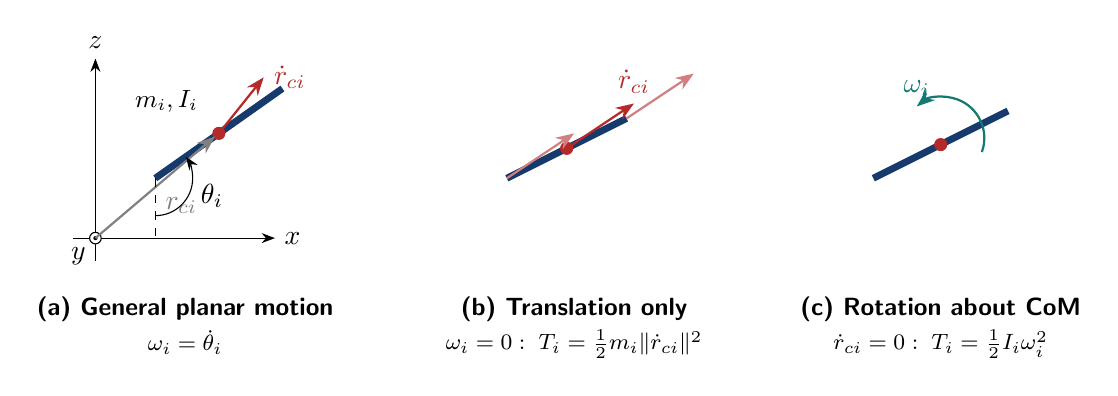
\begin{tikzpicture}[scale=0.95, >=Stealth]
  % Panel (a): General planar motion
  \begin{scope}[shift={(0,0)}]
    \draw[->] (-0.3,0) -- (2.4,0) node[right] {$x$};
    \draw[->] (0,-0.3) -- (0,2.4) node[above] {$z$};
    \filldraw[fill=white, draw=black] (0,0) circle (2.2pt);
    \fill (0,0) circle (0.8pt) node[below left] {$y$};
    % Link
    \draw[line width=2.5pt, navy, rounded corners=2pt] (0.8,0.8) -- (2.5,2.0);
    \fill[accentred] (1.65,1.4) circle (2.5pt);
    \draw[->, thick, gray] (0,0) -- (1.6,1.36) node[midway, below right] {$r_{ci}$};
    \draw[->, thick, accentred] (1.65,1.4) -- (2.25,2.15) node[right] {$\dot{r}_{ci}$};
    \draw[dashed] (0.8,0.8) -- (0.8,0.0);
    \draw[->] (0.8,0.3) arc (-90:35:0.5) node[midway, right, xshift=1pt] {$\theta_i$};
    \node[above left, font=\small] at (1.5,1.55) {$m_i, I_i$};
    \node[below, font=\small\bfseries] at (1.2,-0.65) {(a) General planar motion};
    \node[below, font=\footnotesize] at (1.2,-1.1) {$\omega_i = \dot{\theta}_i$};
  \end{scope}

  % Panel (b): Translation only
  \begin{scope}[shift={(5.0,0)}]
    \draw[line width=2.5pt, navy] (0.5,0.8) -- (2.1,1.6);
    \fill[accentred] (1.3,1.2) circle (2.5pt);
    \draw[->, thick, accentred] (1.3,1.2) -- (2.2,1.8) node[above] {$\dot{r}_{ci}$};
    \draw[->, thick, accentred!60] (0.5,0.8) -- (1.4,1.4);
    \draw[->, thick, accentred!60] (2.1,1.6) -- (3.0,2.2);
    \node[below, font=\small\bfseries] at (1.4,-0.65) {(b) Translation only};
    \node[below, font=\footnotesize] at (1.4,-1.1) {$\omega_i = 0:\; T_i = \frac{1}{2}m_i\|\dot{r}_{ci}\|^2$};
  \end{scope}

  % Panel (c): Rotation about CoM
  \begin{scope}[shift={(10.0,0)}]
    \draw[line width=2.5pt, navy] (0.4,0.8) -- (2.2,1.7);
    \fill[accentred] (1.3,1.25) circle (2.5pt);
    \draw[->, thick, accentteal] (1.85,1.15) arc (-20:130:0.55) node[above] {$\omega_i$};
    \node[below, font=\small\bfseries] at (1.3,-0.65) {(c) Rotation about CoM};
    \node[below, font=\footnotesize] at (1.3,-1.1) {$\dot{r}_{ci} = 0:\; T_i = \frac{1}{2}I_i\omega_i^2$};
  \end{scope}
\end{tikzpicture}
\caption{Decomposition of planar rigid-link kinetic energy into translation of the CoM and rotation about the CoM \emph{(slide 10)}.}
\label{fig:planar_motion}
\end{figure}

\subsection{Euler--Lagrange Equations, Virtual Work, and External Wrenches \emph{(slides 11--16)}}

For each generalized coordinate $q_i$ ($i = 1, \dots, m$), the \textbf{Euler--Lagrange equations} read
\begin{equation}
  \frac{d}{dt}\frac{\partial L}{\partial \dot{q}_i} - \frac{\partial L}{\partial q_i} = Q_i, \qquad i = 1, \dots, m,
  \label{eq:EL}
\end{equation}
where $Q_i$ is the total applied nonconservative generalized force on $q_i$ (from actuators and any external wrenches). Ideal internal constraint reactions at hinges never appear: they are automatically eliminated by choosing independent coordinates.

\begin{definition}[Generalized Forces via Virtual Work and Input Matrix $B(q)$]
For an arbitrary virtual displacement $\delta q \in \mathbb{R}^m$, the virtual work of the actuators defines the generalized actuator force vector $Q_{\text{act}} \in \mathbb{R}^m$:
\[
  \delta W_{\text{act}} = \sum_{i=1}^{m} Q_{\text{act}, i} \delta q_i = Q_{\text{act}}^T \delta q.
\]
Here $Q_i$ has units of torque if $q_i$ is an angle, and force if $q_i$ is a length. When the $p$ actuators act along displacement coordinates $s(q) \in \mathbb{R}^p$ with inputs $u \in \mathbb{R}^p$,
\[
  \delta W_{\text{act}} = u^T \delta s = u^T \frac{\partial s}{\partial q} \delta q
  \quad\Longrightarrow\quad
  Q_{\text{act}} = B(q) u, \qquad B(q) = \left(\frac{\partial s}{\partial q}\right)^T \in \mathbb{R}^{m \times p}.
\]
More generally, even when no displacement function $s(q)$ exists (e.g., a body-fixed thrust), $B(q)$ is defined by equating $\delta W_{\text{act}} = (B(q)u)^T \delta q$ for every $\delta q$.
\end{definition}

\begin{example}[Three Checks on $B(q)$ \emph{(slide 13)}]
\begin{enumerate}[label=\arabic*.]
  \item \textbf{Cart--pendulum}, $q = (x, \theta)^T$: the linear drive moves with the cart, $s = x \Rightarrow B = (1, 0)^T$.
  \item \textbf{Two-link pendulum (relative elbow angle $q_2$)}: an elbow motor turns through $s = q_2 \Rightarrow B = (0, 1)^T$.
  \item \textbf{Same elbow motor (absolute link angles $\theta_1, \theta_2$)}: $s = \theta_2 - \theta_1 \Rightarrow B = (-1, 1)^T$. The motor exerts equal and opposite torques on the two links, yet it is still a single input ($p = 1$).
\end{enumerate}
\end{example}

For an external wrench $w_k = \begin{bmatrix} f_k \\ n_k \end{bmatrix} \in \mathbb{R}^6$ (force $f_k \in \mathbb{R}^3$ and moment $n_k \in \mathbb{R}^3$) applied to a rigid body whose spatial velocity at the application point is $\begin{bmatrix} v_k \\ \omega_k \end{bmatrix} = J_k(q)\dot{q}$ (via the geometric Jacobian $J_k(q) \in \mathbb{R}^{6 \times m}$), virtual work gives
\[
  Q_{\text{ext}, k} = J_k(q)^T w_k,
\]
provided wrench and velocity are expressed in the same frame and the moment is taken about the point whose linear velocity is used.

Since the kinetic energy is quadratic in velocities, $T = \frac{1}{2}\dot{q}^T M(q)\dot{q}$, expanding \eqref{eq:EL} produces the \textbf{standard manipulator form}:
\begin{equation}
  M(q)\ddot{q} + h(q, \dot{q}) + G(q) = B(q)u + \sum_{k=1}^{N_w} J_k(q)^T w_k,
  \label{eq:standard_form}
\end{equation}
where:
\begin{itemize}
  \item $M(q) = M(q)^T \succ 0$ is the symmetric positive-definite \emph{inertia matrix}; its off-diagonal entries $M_{ij}$ encode inertial coupling between coordinates;
  \item $h(q, \dot{q}) = C(q,\dot{q})\dot{q}$ collects \emph{centrifugal and Coriolis terms}, given componentwise by
  \[
    h_i(q, \dot{q}) = \sum_{j,k=1}^{m} \left(\frac{\partial M_{ij}}{\partial q_k} - \frac{1}{2}\frac{\partial M_{jk}}{\partial q_i}\right)\dot{q}_j \dot{q}_k.
  \]
  These terms exist only because $M$ depends on $q$, are quadratic in $\dot{q}$, and vanish at rest. Note that the matrix factorization $C(q,\dot{q})$ is not unique, whereas the vector $h(q,\dot{q})$ is unique.
  \item $G(q) = \frac{\partial V}{\partial q}$ is the gradient of the potential energy.
  \item $B(q) \in \mathbb{R}^{m \times p}$ maps commanded inputs $u$ into generalized forces; $\operatorname{rank} B(q) \le p$ and may drop at actuation singularities.
\end{itemize}
Without external wrenches (all models in this lecture) and neglecting dissipation, we write $M(q)\ddot{q} + h(q,\dot{q}) + G(q) = B(q)u$, or concisely $M(q)\ddot{q} + n(q,\dot{q}) = B(q)u$ with $n = h + G$.

\begin{intuition}
Whether a force belongs in $B(q)u$ or in $J_k^T w_k$ is a \emph{physical} distinction, not a mathematical one. A controlled propeller thrust on a VTOL acts on a rigid body rather than a joint, yet because it is commanded by the controller, it belongs in $B(q)u$.
\end{intuition}

\subsection{Balance Laws: Energy and Momentum (Q2) \emph{(slides 17--18)}}

\begin{proposition}[Energy Balance Law \emph{(slide 17)}]
Along every trajectory of \eqref{eq:standard_form}, the total mechanical energy $E = T + V$ satisfies
\[
  \frac{dE}{dt} = \underbrace{\dot{q}^T B(q) u}_{\text{actuator power}} + \underbrace{\sum_{k=1}^{N_w} w_k^T J_k(q)\dot{q}}_{\text{external-wrench power}}.
\]
Without external wrenches, $\dot{E} = \dot{q}^T B u = u^T B^T \dot{q}$; if actuator displacement coordinates $s(q)$ exist, then $\dot{E} = u^T \dot{s}$.
\end{proposition}

\begin{proof}
Left-multiply \eqref{eq:standard_form} by $\dot{q}^T$. From the formula for $h_i$,
\[
  \dot{q}^T h = \sum_{i,j,k} \frac{\partial M_{ij}}{\partial q_k}\dot{q}_i \dot{q}_j \dot{q}_k - \frac{1}{2}\sum_{i,j,k}\frac{\partial M_{jk}}{\partial q_i}\dot{q}_i \dot{q}_j \dot{q}_k = \frac{1}{2}\dot{q}^T \dot{M} \dot{q},
\]
so $\dot{q}^T(M\ddot{q} + h) = \dot{q}^T M \ddot{q} + \frac{1}{2}\dot{q}^T \dot{M}\dot{q} = \frac{d}{dt}\left(\frac{1}{2}\dot{q}^T M \dot{q}\right) = \frac{dT}{dt}$. Likewise, $\dot{q}^T G(q) = \dot{q}^T \frac{\partial V}{\partial q} = \frac{dV}{dt}$. Adding the two yields $\frac{dE}{dt} = \dot{q}^T B(q)u + \sum_{k=1}^{N_w} w_k^T J_k(q)\dot{q}$.
\end{proof}

\begin{proposition}[Generalized Momentum and Cyclic Coordinates \emph{(slide 18)}]
The generalized momentum conjugate to coordinate $q_i$ is
\[
  p_i = \frac{\partial L}{\partial \dot{q}_i} = \sum_{j=1}^{m} M_{ij}(q)\dot{q}_j,
  \qquad \text{and obeys} \qquad
  \dot{p}_i = \frac{\partial L}{\partial q_i} + Q_i.
\]
If $L$ does not depend explicitly on $q_i$ (i.e., $q_i$ is a \textbf{cyclic coordinate}), then $\dot{p}_i = Q_i$: only the applied generalized force changes $p_i$. If $Q_i = 0$, then $p_i$ is conserved.
\end{proposition}

\begin{intuition}
Gravity and centrifugal/Coriolis terms never create or destroy energy---they only shuffle energy between kinetic and potential forms and between links. Meanwhile, a cyclic coordinate is the signature of a physical symmetry: shifting a cart along a flat track or spinning a balanced wheel on its axle changes neither $T$ nor $V$. Quick test: scan $T$ and $V$ for any coordinate that appears \emph{only} through its velocity $\dot{q}_i$.
\end{intuition}

\subsection{Equilibria (Q3) and Linearization for Small Motions (Q4) \emph{(slides 19--22)}}

\begin{definition}[Equilibrium Configuration]
An equilibrium (without external wrenches) is a pair $(q_e, u_e)$ such that placing the system at $q = q_e$ at rest ($\dot{q} = \ddot{q} = 0$) with constant input $u \equiv u_e$ keeps it there forever. Setting $\dot{q} = \ddot{q} = 0$ in \eqref{eq:standard_form} eliminates $M\ddot{q}$ and $h$, leaving the static balance
\[
  G(q_e) = B(q_e) u_e.
\]
Solutions with $u_e = 0$ are \textbf{natural equilibria} ($\partial V / \partial q = 0$, stationary points of potential energy).
\end{definition}

When $p = m$ (fully actuated, full-rank $B$), every configuration $q_e$ can be held by choosing $u_e = B(q_e)^{-1} G(q_e)$. When $p < m$, only a restricted subset of configurations satisfies $G(q_e) \in \operatorname{Im} B(q_e)$.

\begin{proposition}[Linearized Model About an Equilibrium \emph{(slide 20)}]
Let $q = q_e + \delta q$ and $u = u_e + \delta u$. If $B$ is constant, then to first order in $(\delta q, \delta \dot{q}, \delta u)$,
\begin{equation}
  M_e \delta\ddot{q} + K_e \delta q = B \delta u,
  \qquad M_e = M(q_e), \qquad K_e = \left.\frac{\partial^2 V}{\partial q^2}\right|_{q=q_e}.
  \label{eq:linearized}
\end{equation}
If $B(q)$ depends on $q$, the stiffness matrix generalizes to $K_e = \left.\frac{\partial}{\partial q}\big(G(q) - B(q)u_e\big)\right|_{q=q_e}$, which is not necessarily symmetric.
\end{proposition}

\begin{proof}
Expand each term about $(q_e, u_e)$: $M(q_e + \delta q)\delta\ddot{q} = M_e \delta\ddot{q} + O(\|\delta q\|\|\delta\ddot{q}\|)$; $h(q, \delta\dot{q})$ is quadratic in $\delta\dot{q}$, hence second order; $G(q_e + \delta q) = G(q_e) + K_e \delta q + O(\|\delta q\|^2)$. Using $G(q_e) = B u_e$ cancels the zeroth-order terms, yielding \eqref{eq:linearized}.
\end{proof}

To analyze free small motions ($\delta u = 0$), substitute $\delta q(t) = v e^{st}$ into \eqref{eq:linearized}. This gives the generalized eigenvalue problem
\[
  K_e v = \mu M_e v, \qquad s^2 = -\mu.
\]
When $M_e = M_e^T \succ 0$ and $K_e = K_e^T$, there are $m$ real characteristic values $\mu_i$ with corresponding mode shapes $v_i$, and system eigenvalues $\lambda_{i,\pm} = \pm\sqrt{-\mu_i}$:
\begin{itemize}
  \item $\mu_i > 0$ (\textbf{oscillation}): natural frequency $\omega_i = \sqrt{\mu_i}$, period $2\pi / \omega_i$;
  \item $\mu_i < 0$ (\textbf{unstable fall}): growth/decay rates $\pm\lambda_i$ with $\lambda_i = \sqrt{-\mu_i}$; a deviation grows by a factor $e \approx 2.718$ in time $1/\lambda_i$;
  \item $\mu_i = 0$ (\textbf{drift}): $\delta q(t) = (a + bt) v_i$, along flat directions of $V$.
\end{itemize}

\begin{proposition}[Stability Read from Potential Energy \emph{(slides 21--22)}]
For constant $B$, the signs of the characteristic values $\mu_i$ (and hence the stability type of the undamped linearized system) are determined solely by the Hessian $K_e = \partial^2 V / \partial q^2$ of the potential energy. The inertia matrix $M_e$ determines \emph{how fast} the system oscillates or falls, but not whether it is stable.
\end{proposition}

In first-order state-space form with state $x = (\delta q, \delta\dot{q})^T \in \mathbb{R}^{2m}$, \eqref{eq:linearized} becomes
\[
  \dot{x} = A x + B_\ell \delta u, \qquad
  A = \begin{bmatrix} 0 & I \\ -M_e^{-1} K_e & 0 \end{bmatrix}, \qquad
  B_\ell = \begin{bmatrix} 0 \\ M_e^{-1} B \end{bmatrix}.
\]

\begin{intuition}
Notice that for constant $B$, $K_e$ does not depend on $u_e$: holding a posture with a constant torque does not change how the system reacts to a small nudge! Also remember two cautions: (i) without friction, ``stable'' means marginal stability (perpetual oscillation nearby, not convergence to rest); (ii) this describes an open-loop robot with \emph{no feedback} and holds only for small deviations (it says nothing about swing-up).
\end{intuition}

\subsection{The Seven-Step Modeling Recipe \emph{(slide 23)}}

\begin{algorithm}[Modeling and Reading Recipe \emph{(slide 23)}]
\begin{enumerate}[label=\arabic*.]
  \item Choose independent coordinates $q$; state precisely where each angle is measured from.
  \item Write the CoM positions $r_{ci}(q)$ and differentiate them to get $\dot{r}_{ci}$.
  \item Form $T$ and $V$; read off $M(q)$ from $T = \frac{1}{2}\dot{q}^T M(q)\dot{q}$.
  \item Apply the Euler--Lagrange equation to each coordinate.
  \item Find $B(q)$ from the virtual work of the actuators.
  \item Check the result on limit cases (a locked joint, a mass going to $0$ or $\infty$, zero gravity).
  \item Ask the five structural questions Q1--Q5.
\end{enumerate}
\emph{Steps 1--5 produce the equations; Steps 6--7 produce understanding.}
\end{algorithm}

% ============================================================================
\section{Part 2: Warm-Up --- The Pendulum \emph{(slides 24--28)}}
% ============================================================================

\subsection{Model and Equivalent Length \emph{(slide 25)}}

Consider a rigid body of mass $m_p$ pivoting about a fixed horizontal axis, with CoM at distance $\ell_c$, moment of inertia about the hinge $I_h = I + m_p \ell_c^2$, angle $\theta$ from the downward vertical (CCW), and motor torque $\tau$. Its energies are $T = \frac{1}{2} I_h \dot{\theta}^2$ and $V = -m_p g \ell_c \cos\theta$, giving
\begin{equation}
  I_h \ddot{\theta} + m_p g \ell_c \sin\theta = \tau.
  \label{eq:pendulum}
\end{equation}
Two constants summarize the pendulum's dynamics:
\[
  \omega_0 = \sqrt{\frac{m_p g \ell_c}{I_h}} = \sqrt{\frac{g}{\ell_{\text{eq}}}}, \qquad
  \ell_{\text{eq}} = \frac{I_h}{m_p \ell_c} \quad (\text{equivalent length}).
\]
With the reference values ($m_p = 0.5\,\mathrm{kg}$, $\ell_c = 0.4\,\mathrm{m}$, point mass), we get $\ell_{\text{eq}} = 0.4\,\mathrm{m}$ and $\omega_0 = 4.95\,\mathrm{rad/s}$. With a motor ($p=m=1$) it is fully actuated; without ($\tau \equiv 0$, $p=0$) it is the simplest passive coordinate. For $m=1$, Q1 and Q5 are vacuous.

\subsection{All Motions in One Picture (Q2, Q3) \emph{(slide 26)}}

\begin{itemize}
  \item \textbf{Q2 (Energy, $\tau=0$):} $E = \frac{1}{2}I_h \dot{\theta}^2 - m_p g \ell_c \cos\theta$ is conserved. Every trajectory follows a level curve of $E$: closed \emph{oscillations} ($E < m_p g \ell_c$), open \emph{rotations} ($E > m_p g \ell_c$), and between them the \textbf{separatrix} ($E = m_p g \ell_c$):
  \[
    \dot{\theta} = \pm 2\omega_0 \cos(\theta / 2).
  \]
  The separatrix is the homoclinic orbit of the upright position: along it, the pendulum approaches the top in infinite time. This immediately inspires energy-based swing-up control: pump energy until $E = m_p g \ell_c$.
  \item \textbf{Q3 (Equilibria with constant torque):} $m_p g \ell_c \sin\theta_e = \tau_e$. For $|\tau_e| < m_p g \ell_c$, there are two equilibria (one below the horizontal, one above), merging at $\theta_e = \pm 90^\circ$ when $|\tau_e| = m_p g \ell_c$, and none for $|\tau_e| > m_p g \ell_c$. With $m_p g \ell_c = 1.96\,\mathrm{Nm}$, a motor limited to $1.5\,\mathrm{Nm}$ can hold the pendulum only up to $\theta_e = \arcsin(1.5/1.96) = 49.9^\circ$.
\end{itemize}

\begin{figure}[ht]
\centering
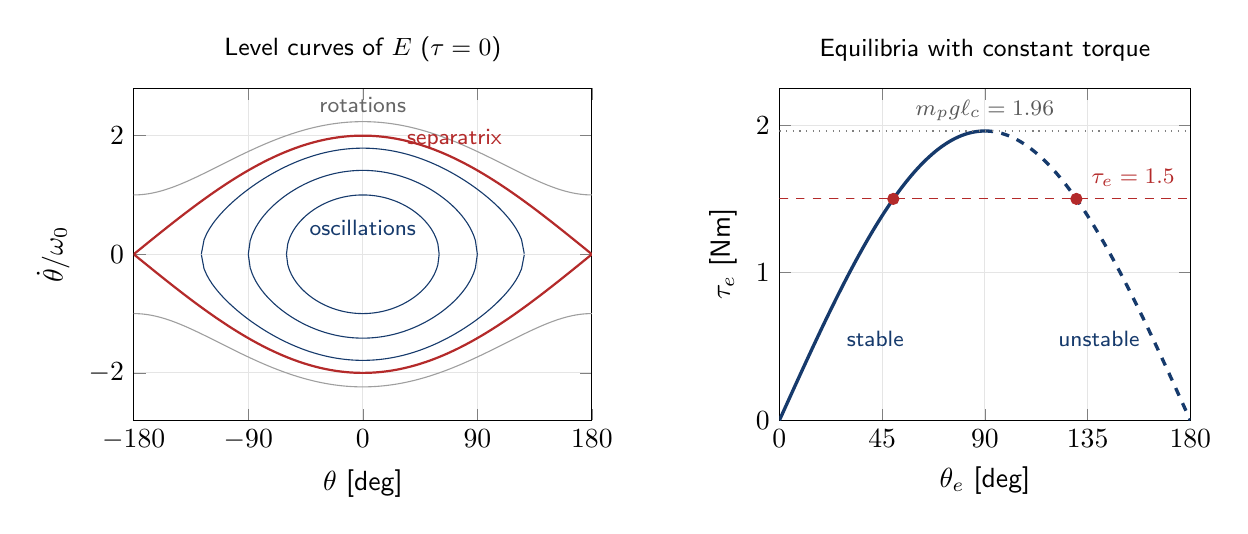
\begin{tikzpicture}
  % Left plot: Phase portrait (energy level curves)
  \begin{axis}[
    width=7.4cm, height=5.8cm,
    title={\small Level curves of $E$ ($\tau = 0$)},
    xlabel={$\theta$ [deg]}, ylabel={$\dot{\theta}/\omega_0$},
    xmin=-180, xmax=180, ymin=-2.8, ymax=2.8,
    xtick={-180,-90,0,90,180}, ytick={-2,0,2},
    grid=major, grid style={gray!20},
    samples=120
  ]
    % Separatrix: +/- 2 cos(theta/2)
    \addplot[thick, accentred, domain=-180:180] {2*cos(x/2)};
    \addplot[thick, accentred, domain=-180:180] {-2*cos(x/2)};
    % Oscillations: E/(mpg lc) = -0.5, 0.0, 0.6 -> (thetadot/w0)^2 = 2(e + cos(theta))
    \addplot[navy, domain=-60:60] {sqrt(max(0, 2*(-0.5 + cos(x))))};
    \addplot[navy, domain=-60:60] {-sqrt(max(0, 2*(-0.5 + cos(x))))};
    \addplot[navy, domain=-90:90] {sqrt(max(0, 2*(0.0 + cos(x))))};
    \addplot[navy, domain=-90:90] {-sqrt(max(0, 2*(0.0 + cos(x))))};
    \addplot[navy, domain=-126.87:126.87] {sqrt(max(0, 2*(0.6 + cos(x))))};
    \addplot[navy, domain=-126.87:126.87] {-sqrt(max(0, 2*(0.6 + cos(x))))};
    % Rotations: e = 1.5, 2.2
    \addplot[gray!75, domain=-180:180] {sqrt(2*(1.5 + cos(x)))};
    \addplot[gray!75, domain=-180:180] {-sqrt(2*(1.5 + cos(x)))};
    \node[font=\footnotesize, navy] at (axis cs:0,0.45) {oscillations};
    \node[font=\footnotesize, accentred] at (axis cs:72,1.95) {separatrix};
    \node[font=\footnotesize, gray!80!black] at (axis cs:0,2.52) {rotations};
  \end{axis}

  % Right plot: Static equilibria tau_e = mpg lc sin(theta_e)
  \begin{axis}[
    xshift=8.2cm,
    width=6.8cm, height=5.8cm,
    title={\small Equilibria with constant torque},
    xlabel={$\theta_e$ [deg]}, ylabel={$\tau_e$ [Nm]},
    xmin=0, xmax=180, ymin=0, ymax=2.25,
    xtick={0,45,90,135,180}, ytick={0,1,2},
    grid=major, grid style={gray!20},
    samples=100
  ]
    \addplot[very thick, navy, domain=0:90] {1.96*sin(x)};
    \addplot[very thick, navy, dashed, domain=90:180] {1.96*sin(x)};
    \addplot[dashed, accentred, domain=0:180] {1.5};
    \addplot[dotted, gray, domain=0:180] {1.96};
    \addplot[only marks, mark=*, accentred, mark size=2pt] coordinates {(49.9, 1.5) (130.1, 1.5)};
    \node[font=\footnotesize, above, gray!70!black] at (axis cs:90,1.96) {$m_p g \ell_c = 1.96$};
    \node[font=\footnotesize, above, accentred] at (axis cs:155,1.52) {$\tau_e = 1.5$};
    \node[font=\footnotesize, navy] at (axis cs:42,0.55) {stable};
    \node[font=\footnotesize, navy] at (axis cs:140,0.55) {unstable};
  \end{axis}
\end{tikzpicture}
\caption{Left: Pendulum energy level curves in the $(\theta, \dot{\theta}/\omega_0)$ phase plane for $\tau=0$. Right: Constant-torque equilibrium curve $\tau_e = m_p g \ell_c \sin\theta_e$ showing the stable branch ($0^\circ$--$90^\circ$) and unstable branch ($90^\circ$--$180^\circ$) \emph{(slide 26)}.}
\label{fig:pendulum_phase}
\end{figure}

\subsection{Small Motions (Q4) and Key Numbers \emph{(slides 27--28)}}

Linearizing \eqref{eq:pendulum} about $\theta_e$ gives $M_e = I_h$ and $K_e = m_p g \ell_c \cos\theta_e$, yielding a single characteristic value
\[
  \mu = \omega_0^2 \cos\theta_e.
\]
Thus, any equilibrium below the horizontal ($\cos\theta_e > 0$) is stable, and any equilibrium above the horizontal ($\cos\theta_e < 0$) is unstable, \emph{regardless of the constant torque holding it}:
\begin{itemize}
  \item \textbf{Hanging ($\theta_e = 0$):} oscillations at $\omega_0 = 4.95\,\mathrm{rad/s}$ (period $1.27\,\mathrm{s}$).
  \item \textbf{Held below horizontal:} $\omega = \omega_0 \sqrt{\cos\theta_e}$ ($3.98\,\mathrm{rad/s}$ at $49.9^\circ$); gravity acts as a softer spring.
  \item \textbf{Upright ($\theta_e = \pi$):} $\delta\theta(t) = \delta\theta(0)\cosh(\lambda t)$ with $\lambda = \omega_0 = 4.95\,\mathrm{s}^{-1}$, time constant $1/\lambda = 0.20\,\mathrm{s}$. Released $1^\circ$ from the top, it reaches $1.5^\circ$ after $0.2\,\mathrm{s}$, $3.7^\circ$ after $0.4\,\mathrm{s}$, and $9.8^\circ$ after $0.6\,\mathrm{s}$.
\end{itemize}

\begin{intuition}[Broom vs.\ Pencil, Linear Range, and Discussion]
Since $\lambda = \sqrt{g / \ell_{\text{eq}}}$, a longer inverted object falls more slowly: a broom is far easier to balance on your hand than a pencil. How far is ``linear''? The true nonlinear period exceeds the linearized period by $+1.7\%$ at $30^\circ$, $+7\%$ at $60^\circ$, and $+18\%$ at $90^\circ$.

\medskip
\noindent\textbf{Three numbers to remember for a pendulum:} (1) $\omega_0 = \sqrt{g/\ell_{\text{eq}}}$ (oscillation frequency and upright fall rate); (2) $m_p g \ell_c$ (peak gravity torque a motor must exceed to hold any angle); (3) $2 m_p g \ell_c$ (energy separating bottom from top: $3.9\,\mathrm{J}$ for reference values).

\medskip
\noindent\textbf{Discussion (slide 28):} Drawing the phase portrait without solving the ODE was possible because the 1-DoF system has a conserved quantity $E(\theta,\dot{\theta})$ whose level curves are 1D curves in the 2D phase plane. With hinge friction, $\dot{E} = -b\dot{\theta}^2 \le 0$, so trajectories cross level curves inward toward the bottom equilibrium rather than following them.
\end{intuition}

% ============================================================================
\section{Part 3: The Cart--Pendulum \emph{(slides 29--41)}}
% ============================================================================

\subsection{Geometry, Energies, and Dynamic Model (Q1) \emph{(slides 30--31)}}

Let $q = (x, \theta)^T$, where $x$ is the horizontal position of the cart (mass $M$) and $\theta$ is the pole angle measured \emph{clockwise from the upward vertical}. A horizontal force $F$ pushes the cart; the hinge at height $z_0$ is passive. The pole CoM position is $r_G = (x + \ell_c \sin\theta,\, 0,\, z_0 + \ell_c \cos\theta)^T$. Differentiating gives $\dot{r}_G = (\dot{x} + \ell_c \cos\theta\,\dot{\theta},\, 0,\, -\ell_c \sin\theta\,\dot{\theta})^T$, so with $I_h = I + m_p \ell_c^2$:
\[
  T = \frac{1}{2}(M + m_p)\dot{x}^2 + m_p \ell_c \cos\theta\,\dot{x}\dot{\theta} + \frac{1}{2} I_h \dot{\theta}^2, \qquad
  V = m_p g \ell_c \cos\theta, \qquad
  \delta W = F \delta x.
\]

\begin{figure}[ht]
\centering
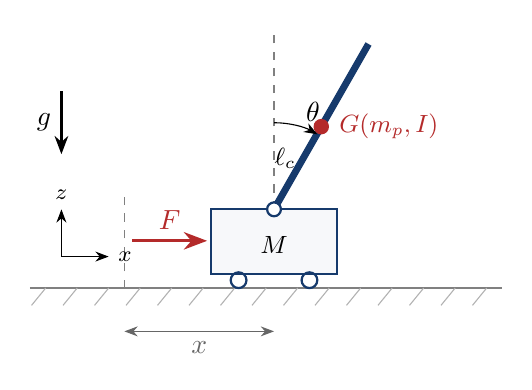
\begin{tikzpicture}[scale=1.0, >=Stealth]
  % Track
  \draw[thick, gray] (-1.2,0) -- (4.8,0);
  \foreach \x in {-1.0,-0.6,...,4.6} {
    \draw[gray!60] (\x,0) -- (\x-0.18,-0.22);
  }
  % Cart
  \draw[thick, fill=thmbg, draw=navy] (1.1,0.18) rectangle (2.7,1.0);
  \draw[thick, navy] (1.45,0.1) circle (0.1);
  \draw[thick, navy] (2.35,0.1) circle (0.1);
  \node[font=\small] at (1.9,0.55) {$M$};
  % Force F
  \draw[->, very thick, accentred] (0.1,0.6) -- (1.05,0.6) node[midway, above] {$F$};
  % x coordinate
  \draw[dashed, gray] (0,0) -- (0,1.2);
  \draw[<->, gray!80!black] (0,-0.55) -- (1.9,-0.55) node[midway, below] {$x$};
  % Pole
  \draw[dashed, gray] (1.9,1.0) -- (1.9,3.3);
  \draw[line width=2.5pt, navy] (1.9,1.0) -- (3.1,3.1);
  \fill[white, draw=navy, thick] (1.9,1.0) circle (2.5pt);
  \fill[accentred] (2.5,2.05) circle (2.8pt) node[right, xshift=3pt, font=\small] {$G(m_p, I)$};
  \draw[->] (1.9,2.1) arc (90:60:1.1) node[midway, above right, yshift=-2pt] {$\theta$};
  \node[left, font=\small] at (2.3,1.65) {$\ell_c$};
  % Gravity & axes
  \draw[->, thick] (-0.8,2.5) -- (-0.8,1.7) node[midway, left] {$g$};
  \draw[->] (-0.8,0.4) -- (-0.2,0.4) node[right, font=\footnotesize] {$x$};
  \draw[->] (-0.8,0.4) -- (-0.8,1.0) node[above, font=\footnotesize] {$z$};
\end{tikzpicture}
\caption{Cart--pendulum geometry: $\theta$ is measured clockwise from the upward vertical \emph{(slide 30)}.}
\label{fig:cart_pendulum}
\end{figure}

Applying the Euler--Lagrange equations yields the cart--pendulum dynamic model:
\begin{equation}
  \begin{bmatrix} M + m_p & m_p \ell_c \cos\theta \\ m_p \ell_c \cos\theta & I_h \end{bmatrix}
  \begin{bmatrix} \ddot{x} \\ \ddot{\theta} \end{bmatrix}
  + \begin{bmatrix} -m_p \ell_c \sin\theta\,\dot{\theta}^2 \\ -m_p g \ell_c \sin\theta \end{bmatrix}
  = \begin{bmatrix} F \\ 0 \end{bmatrix}.
  \label{eq:cart_pendulum}
\end{equation}
Notice that $\det M(\theta) = (M + m_p)I + M m_p \ell_c^2 + m_p^2 \ell_c^2 \sin^2\theta > 0$ everywhere, so accelerations are always well-defined.

\textbf{Q1 (Structure):} The two rows play completely different roles:
\begin{itemize}
  \item \emph{Row 1} contains the input $F$: it is Newton's second law for the horizontal motion of the whole system.
  \item \emph{Row 2} has no input. Dividing by $m_p \ell_c$ gives
  \[
    \ddot{\theta} = \frac{1}{\ell_{\text{eq}}} \big( g\sin\theta - \ddot{x}\cos\theta \big), \qquad \ell_{\text{eq}} = \frac{I_h}{m_p \ell_c} = 0.4\,\mathrm{m}.
  \]
  The pole behaves exactly as a pendulum of length $\ell_{\text{eq}}$ whose pivot is accelerated horizontally. The force $F$ reaches the pole \emph{only} through $\ddot{x}$.
\end{itemize}

\subsection{Momentum and Recoil (Q2) \emph{(slide 32)}}

\begin{itemize}
  \item \textbf{Energy:} $\dot{E} = F \dot{x}$. The force changes mechanical energy only while the cart is moving.
  \item \textbf{Cyclic coordinate $x$:} Neither $T$ nor $V$ contains $x$. Its conjugate momentum is
  \[
    p_x = (M + m_p)\dot{x} + m_p \ell_c \cos\theta\,\dot{\theta} = (M + m_p)\dot{x}_G, \qquad \dot{p}_x = F,
  \]
  where $x_G = x + \frac{m_p \ell_c}{M + m_p}\sin\theta$ is the horizontal coordinate of the overall CoM.
\end{itemize}

\begin{intuition}[Recoil Without Force]
When $F = 0$ and the system starts from rest, $p_x \equiv 0$, so the overall CoM $x_G$ cannot move horizontally:
\[
  x(t) = x_G - \frac{m_p \ell_c}{M + m_p}\sin\theta(t).
\]
As the pole falls to the right ($\sin\theta$ increases), the cart must recoil to the left. With the reference values ($M=1\,\mathrm{kg}$, $m_p=0.2\,\mathrm{kg}$, $\ell_c=0.3\,\mathrm{m}$), the maximum recoil is $\frac{0.2 \times 0.3}{1.2} = 0.05\,\mathrm{m} = 5\,\mathrm{cm}$.
\end{intuition}

\subsection{Equilibria and Constant-Inclination Motions (Q3) \emph{(slides 33--35)}}

With $G = (0, -m_p g \ell_c \sin\theta)^T$ and $B = (1, 0)^T$, the static equilibrium condition $G(q_e) = B F_e$ yields
\[
  F_e = 0, \qquad \sin\theta_e = 0.
\]
\begin{itemize}
  \item \textbf{Static equilibria:} Two one-parameter families---pole up ($\theta_e = 0$) or pole down ($\theta_e = \pi$), with the cart at any position $x_e$ (since $V$ does not depend on $x$).
  \item \textbf{Relative equilibria (uniform translation):} $x(t) = x_0 + v_0 t$, $\theta(t) \in \{0, \pi\}$, $F = 0$. The upright configuration remains unstable.
  \item \textbf{Pole on a free cart ($F = 0$):} Eliminating $\ddot{x}$ from Row 1 into Row 2 gives a single scalar ODE for the pole:
  \[
    \left(I_h - \frac{m_p^2 \ell_c^2 \cos^2\theta}{M + m_p}\right)\ddot{\theta}
    + \frac{m_p^2 \ell_c^2}{M + m_p}\sin\theta\cos\theta\,\dot{\theta}^2
    - m_p g \ell_c \sin\theta = 0.
  \]
  Because the cart recoils horizontally as the pole rotates, the pole experiences a \emph{smaller, angle-dependent effective inertia}.
  \item \textbf{Constant-inclination forced trajectory:} The pole cannot rest statically at a nonvertical angle $\bar{\theta}$ under any constant force, because a constant force simply accelerates the cart. However, setting $\theta(t) \equiv \bar{\theta}$ ($\dot{\theta} = \ddot{\theta} = 0$) in Row 2 gives $\ddot{x} = g\tan\bar{\theta}$, which requires the constant force $F = (M + m_p)g\tan\bar{\theta}$ and yields the uniformly accelerating trajectory
  \[
    x(t) = x_0 + v_0 t + \frac{1}{2} g \tan\bar{\theta}\, t^2, \qquad \theta(t) = \bar{\theta}.
  \]
  In the accelerating cart frame, the inertial force balances the gravitational torque on the inclined pole.
\end{itemize}

\subsection{Small Motions, Linear Model, and the ``Wrong-Way'' Zero (Q4) \emph{(slides 36--39)}}

About $\theta_e \in \{0, \pi\}$, $K_e = \operatorname{diag}(0,\, -m_p g \ell_c \cos\theta_e)$ and $M_e = \begin{bmatrix} M+m_p & \pm m_p \ell_c \\ \pm m_p \ell_c & I_h \end{bmatrix}$ with $\Delta_0 = \det M_e = (M+m_p)I_h - m_p^2 \ell_c^2$. The characteristic values are $\mu_1 = 0$ (cart drift) and $\mu_2 = \mp (M+m_p)m_p g \ell_c / \Delta_0$. For the upright pole ($\theta_e = 0$), the instability rate is
\[
  \lambda = \sqrt{\frac{(M + m_p) m_p g \ell_c}{\Delta_0}} = \omega_0 \sqrt{\frac{(M + m_p) I_h}{\Delta_0}} > \omega_0.
\]
With the reference values, $\lambda = 5.29\,\mathrm{s}^{-1}$, strictly faster than $\omega_0 = 4.95\,\mathrm{s}^{-1}$ on a fixed pivot: the cart gives way under the falling pole.

Solving the upright linearized equations for accelerations gives
\[
  \delta\ddot{x} = \frac{I_h \delta F - m_p^2 \ell_c^2 g \delta\theta}{\Delta_0} = 0.952\,\delta F - 1.40\,\delta\theta, \qquad
  \delta\ddot{\theta} = \frac{(M+m_p)m_p g \ell_c \delta\theta - m_p \ell_c \delta F}{\Delta_0} = 28.0\,\delta\theta - 2.38\,\delta F.
\]
Read the signs: pushing the cart right ($\delta F > 0$) tips the pole left ($\delta\ddot{\theta} < 0$, it is left behind); a pole leaning right ($\delta\theta > 0$) pushes the cart left ($\delta\ddot{x} < 0$, recoil). In state-space form with $x = (\delta x, \delta\theta, \delta\dot{x}, \delta\dot{\theta})^T$:
\[
  A = \begin{bmatrix} 0 & 0 & 1 & 0 \\ 0 & 0 & 0 & 1 \\ 0 & -1.40 & 0 & 0 \\ 0 & 28.0 & 0 & 0 \end{bmatrix}, \qquad
  B_\ell = \begin{bmatrix} 0 \\ 0 \\ 0.952 \\ -2.38 \end{bmatrix}.
\]

Eliminating $\delta\theta$ in the Laplace domain gives the force-to-cart-position transfer function:
\[
  \frac{\delta x(s)}{\delta F(s)} = \frac{I_h s^2 - m_p g \ell_c}{s^2 \big(\Delta_0 s^2 - (M + m_p) m_p g \ell_c\big)}.
\]
The denominator reveals the double integrator ($s^2$, cart drift) and the poles $\pm\lambda$. The numerator has zeros at $s = \pm\omega_0$---the fixed-pivot pendulum rates---one of which lies in the open right-half plane.

\begin{intuition}[The ``Wrong-Way'' Zero]
A right-half-plane (non-minimum-phase) zero is the linear signature of an intuitive physical fact: to transport the cart to the right while keeping the pole upright at both start and finish, the cart must \emph{first move to the left} to lean the pole forward, then accelerate right to catch it. Zeros capture the internal dynamics when the output $\delta x$ is held fixed---which here is just the pole on a fixed pivot!
\end{intuition}

When the pole is released from rest at $\theta(0) = 5^\circ$ with $F = 0$:
\begin{enumerate}[label=\arabic*.]
  \item \emph{Slow, then sudden:} it takes $0.25\,\mathrm{s}$ to grow from $5^\circ$ to $10^\circ$, and $0.70\,\mathrm{s}$ to reach horizontal ($90^\circ$), driven by $\lambda = 5.29\,\mathrm{s}^{-1}$.
  \item \emph{Recoil:} the cart moves $4.6\,\mathrm{cm}$ to the left by the time the pole is horizontal, while $x_G$ stays fixed. At $\theta = 90^\circ$, $\cos\theta = 0$ in $p_x = 0$, so the cart instantaneously comes to rest.
  \item \emph{Validity of linearization:} accurate up to $\sim 30^\circ$ ($0.468\,\mathrm{s}$ linear vs.\ $0.471\,\mathrm{s}$ nonlinear); at true $\theta = 60^\circ$, the linear model predicts $63.6^\circ$.
\end{enumerate}

\begin{figure}[ht]
\centering
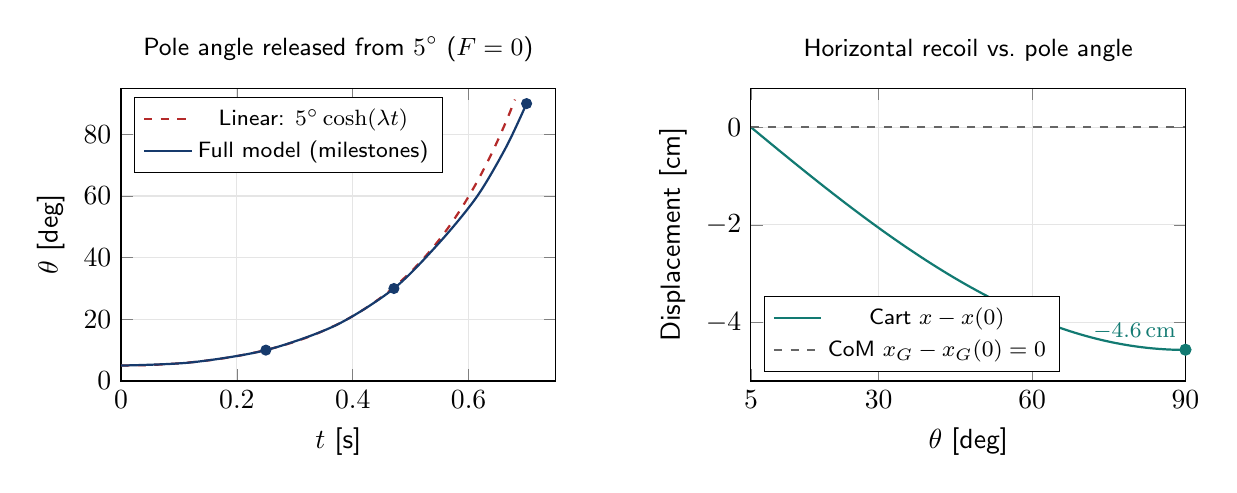
\begin{tikzpicture}
  % Left: Linear vs nonlinear milestones
  \begin{axis}[
    width=7.1cm, height=5.3cm,
    title={\small Pole angle released from $5^\circ$ ($F=0$)},
    xlabel={$t$ [s]}, ylabel={$\theta$ [deg]},
    xmin=0, xmax=0.75, ymin=0, ymax=95,
    xtick={0,0.2,0.4,0.6}, ytick={0,20,40,60,80},
    grid=major, grid style={gray!20},
    legend pos=north west, legend style={font=\footnotesize}
  ]
    \addplot[thick, dashed, accentred, domain=0:0.68, samples=80] {5*0.5*(exp(5.29*x) + exp(-5.29*x))};
    \addlegendentry{Linear: $5^\circ\cosh(\lambda t)$}
    \addplot[thick, navy, smooth] coordinates {
      (0, 5) (0.12, 6.0) (0.25, 10.0) (0.37, 18.0) (0.471, 30.0) (0.55, 45.0) (0.615, 60.0) (0.665, 76.0) (0.70, 90.0)
    };
    \addlegendentry{Full model (milestones)}
    \addplot[only marks, mark=*, navy, mark size=1.8pt] coordinates {(0.25,10) (0.471,30) (0.70,90)};
  \end{axis}

  % Right: Horizontal recoil vs pole angle
  \begin{axis}[
    xshift=8.0cm,
    width=7.1cm, height=5.3cm,
    title={\small Horizontal recoil vs.\ pole angle},
    xlabel={$\theta$ [deg]}, ylabel={Displacement [cm]},
    xmin=5, xmax=90, ymin=-5.2, ymax=0.8,
    xtick={5,30,60,90}, ytick={0,-2,-4},
    grid=major, grid style={gray!20},
    legend pos=south west, legend style={font=\footnotesize}
  ]
    \addplot[thick, accentteal, domain=5:90, samples=80] {-5*(sin(x) - sin(5))};
    \addlegendentry{Cart $x - x(0)$}
    \addplot[thick, dashed, gray!80!black, domain=5:90] {0};
    \addlegendentry{CoM $x_G - x_G(0) = 0$}
    \addplot[only marks, mark=*, accentteal, mark size=2pt] coordinates {(90, -4.56)};
    \node[font=\footnotesize, above left, accentteal] at (axis cs:90,-4.56) {$-4.6\,\mathrm{cm}$};
  \end{axis}
\end{tikzpicture}
\caption{Free fall of the cart--pendulum from $\theta(0)=5^\circ$ with $F=0$: comparison of linear exponential growth with full-model milestones (left), and exact horizontal cart recoil from momentum conservation (right) \emph{(slide 39)}.}
\label{fig:cart_fall}
\end{figure}

\subsection{Coupling, Limit Checks (Q5), and Discussion \emph{(slides 40--41)}}

\textbf{Q5 (Coupling):} The input reaches the pole through the off-diagonal inertia $M_{12}(\theta) = m_p \ell_c \cos\theta$. It is largest when the pole is vertical ($\theta = 0, \pi$), \emph{vanishes} when the pole is horizontal ($\theta = \pm\pi/2$, where pushing the cart cannot exert any torque on the pole), and reverses sign beyond horizontal.

\textbf{Limit checks:} (i) $M \to \infty$ recovers the fixed-pivot upright pendulum; (ii) $m_p \to 0$ gives $M\ddot{x} = F$; (iii) $g = 0$ shows the pole's angular momentum about the hinge changes solely through hinge acceleration $\ddot{x}$.

\begin{intuition}[Discussion: The Massless-Cart Limit $M \to 0$ \emph{(slide 41)}]
For a uniform rod of length $L$ ($\ell_c = L/2$, $I_h = \frac{1}{3}m_p L^2$), as $M \to 0$ we have $\Delta_0 \to m_p I_h - m_p^2 \ell_c^2 = m_p I = \frac{1}{12}m_p^2 L^2$, so
\[
  \frac{(M + m_p) I_h}{\Delta_0} \longrightarrow \frac{m_p \cdot \frac{1}{3}m_p L^2}{\frac{1}{12}m_p^2 L^2} = 4
  \quad\Longrightarrow\quad
  \lambda \longrightarrow 2\omega_0.
\]
With no cart mass to resist horizontal motion, the horizontal position of the CoM stays fixed ($x_G = \text{const}$), so the rod falls by rotating purely about its CoM (inertia $I = I_h / 4$) rather than about its base! One-quarter the inertia means twice the fall rate.
\end{intuition}

% ============================================================================
\section{Part 4: The Two-Link Pendulum --- Acrobot and Pendubot \emph{(slides 42--57)}}
% ============================================================================

\subsection{Conventions, Energies, and Dynamic Model \emph{(slides 43--45)}}

Two rigid links of masses $m_1, m_2$, lengths $\ell_1, \ell_2$, CoM distances $\ell_{c1}, \ell_{c2}$ from their proximal joints, and CoM inertias $I_1, I_2$ form a planar double pendulum. We use $q_1$ (angle of link 1 from the downward vertical, CCW) and $q_2$ (relative elbow angle of link 2 with respect to link 1, CCW), so the absolute angle of link 2 is $q_1 + q_2$.
\begin{itemize}
  \item \textbf{Acrobot:} motor torque $\tau$ at joint 2 (elbow); joint 1 (shoulder) is passive.
  \item \textbf{Pendubot:} motor torque $\tau$ at joint 1 (shoulder); joint 2 (elbow) is passive.
\end{itemize}

\begin{figure}[ht]
\centering
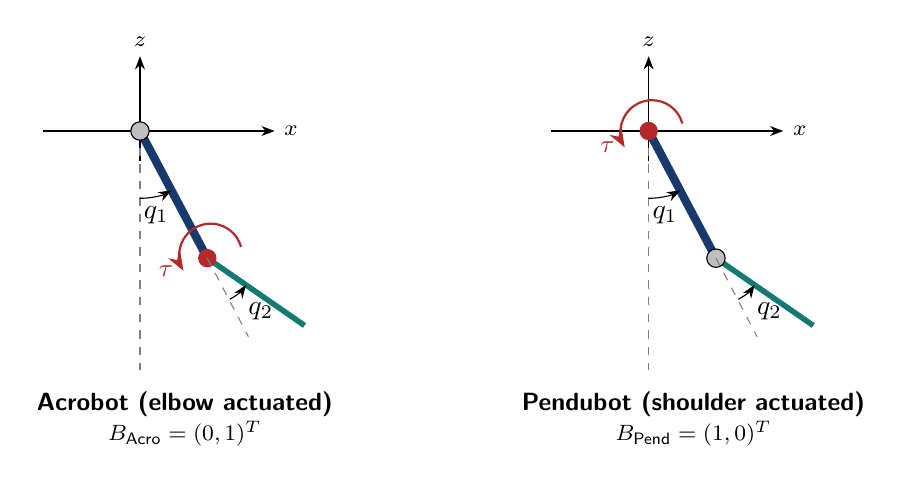
\begin{tikzpicture}[scale=0.95, >=Stealth]
  % Acrobot
  \begin{scope}[shift={(0,0)}]
    \draw[->] (-1.3,0) -- (1.8,0) node[right, font=\footnotesize] {$x$};
    \draw[->] (0,-0.4) -- (0,1.0) node[above, font=\footnotesize] {$z$};
    \draw[dashed, gray] (0,0) -- (0,-3.2);
    % Link 1
    \draw[line width=3pt, navy] (0,0) -- (0.9,-1.7);
    \fill[gray!50, draw=black] (0,0) circle (3.5pt);
    % Link 2
    \draw[line width=2pt, accentteal] (0.9,-1.7) -- (2.2,-2.6);
    \fill[accentred] (0.9,-1.7) circle (3.5pt);
    % Angles
    \draw[->] (0,-0.9) arc (-90:-62:0.9) node[midway, below] {$q_1$};
    \draw[dashed, gray] (0.9,-1.7) -- (1.45,-2.75);
    \draw[->] (1.2,-2.25) arc (-62:-35:0.62) node[midway, below right] {$q_2$};
    % Torque at elbow
    \draw[->, thick, accentred] (1.35,-1.55) arc (15:210:0.42) node[left, font=\small] {$\tau$};
    \node[below, font=\small\bfseries] at (0.6,-3.35) {Acrobot (elbow actuated)};
    \node[below, font=\footnotesize] at (0.6,-3.75) {$B_{\text{Acro}} = (0,1)^T$};
  \end{scope}

  % Pendubot
  \begin{scope}[shift={(6.8,0)}]
    \draw[->] (-1.3,0) -- (1.8,0) node[right, font=\footnotesize] {$x$};
    \draw[->] (0,-0.4) -- (0,1.0) node[above, font=\footnotesize] {$z$};
    \draw[dashed, gray] (0,0) -- (0,-3.2);
    % Link 1
    \draw[line width=3pt, navy] (0,0) -- (0.9,-1.7);
    \fill[accentred] (0,0) circle (3.5pt);
    % Link 2
    \draw[line width=2pt, accentteal] (0.9,-1.7) -- (2.2,-2.6);
    \fill[gray!50, draw=black] (0.9,-1.7) circle (3.5pt);
    % Angles
    \draw[->] (0,-0.9) arc (-90:-62:0.9) node[midway, below] {$q_1$};
    \draw[dashed, gray] (0.9,-1.7) -- (1.45,-2.75);
    \draw[->] (1.2,-2.25) arc (-62:-35:0.62) node[midway, below right] {$q_2$};
    % Torque at shoulder
    \draw[->, thick, accentred] (0.45,0.1) arc (15:210:0.42) node[left, font=\small] {$\tau$};
    \node[below, font=\small\bfseries] at (0.6,-3.35) {Pendubot (shoulder actuated)};
    \node[below, font=\footnotesize] at (0.6,-3.75) {$B_{\text{Pend}} = (1,0)^T$};
  \end{scope}
\end{tikzpicture}
\caption{One mechanism, two robots: the Acrobot (red motor at elbow) and the Pendubot (red motor at shoulder) \emph{(slide 43)}.}
\label{fig:acrobot_pendubot}
\end{figure}

Using the unit vector $e(\alpha) = (\sin\alpha, 0, -\cos\alpha)^T$ along a link at angle $\alpha$ and its derivative $t(\alpha) = de/d\alpha$ (which satisfies $t(\alpha)^T t(\beta) = \cos(\alpha - \beta)$), the CoM positions are $r_{c1} = \ell_{c1} e(q_1)$ and $r_{c2} = \ell_1 e(q_1) + \ell_{c2} e(q_1 + q_2)$, with angular rates $\omega_1 = \dot{q}_1$ and $\omega_2 = \dot{q}_1 + \dot{q}_2$. The kinetic energy is $T = \frac{1}{2}\dot{q}^T M(q_2)\dot{q}$ with
\begin{align*}
  M_{11}(q_2) &= I_1 + m_1 \ell_{c1}^2 + I_2 + m_2 \big(\ell_1^2 + \ell_{c2}^2 + 2\ell_1 \ell_{c2} \cos q_2\big), \\
  M_{12}(q_2) &= I_2 + m_2 \big(\ell_{c2}^2 + \ell_1 \ell_{c2} \cos q_2\big), \qquad
  M_{22} = I_2 + m_2 \ell_{c2}^2.
\end{align*}
The potential energy and gravity vector are
\[
  V(q) = -a \cos q_1 - b \cos(q_1 + q_2), \qquad
  G(q) = \begin{bmatrix} a\sin q_1 + b\sin(q_1 + q_2) \\ b\sin(q_1 + q_2) \end{bmatrix},
\]
where $a = g(m_1 \ell_{c1} + m_2 \ell_1)$ and $b = g m_2 \ell_{c2}$. Defining $\beta(q_2) = m_2 \ell_1 \ell_{c2} \sin q_2$ (so $\partial M_{11}/\partial q_2 = -2\beta$ and $\partial M_{12}/\partial q_2 = -\beta$), the dynamic model is
\begin{equation}
  M(q_2)\ddot{q}
  + \underbrace{\begin{bmatrix} -\beta(q_2)\big(2\dot{q}_1\dot{q}_2 + \dot{q}_2^2\big) \\ \beta(q_2)\dot{q}_1^2 \end{bmatrix}}_{h(q,\dot{q})}
  + G(q) = B u,
  \qquad
  B_{\text{Acro}} = \begin{bmatrix} 0 \\ 1 \end{bmatrix}, \quad
  B_{\text{Pend}} = \begin{bmatrix} 1 \\ 0 \end{bmatrix}.
  \label{eq:twolink}
\end{equation}
With the reference values (Table~\ref{tab:ref_values}), $M_{11} = 0.090 + 0.045\cos q_2$, $M_{12} = 0.015 + 0.0225\cos q_2$, $M_{22} = 0.015\,\mathrm{kg\,m^2}$, $a = 2.943\,\mathrm{Nm}$, and $b = 0.736\,\mathrm{Nm}$.

\subsection{Structure (Q1), Energy, and Momentum (Q2) \emph{(slides 46--48)}}

\begin{itemize}
  \item \textbf{Q1 (Structure):} $M$ depends \emph{only} on the elbow angle $q_2$---rotating the whole arm about the shoulder does not change its inertia, while bending the elbow does. All velocity terms carry $\beta \propto \sin q_2$, vanishing when the arm is straight ($q_2=0$) or folded ($q_2=\pi$). Physically, $G_2$ is the gravitational torque of link 2 about the elbow, while $G_1 = g(m_1 + m_2) x_G$ is the total gravitational torque about the shoulder, where $x_G$ is the horizontal coordinate of the overall CoM.
  \item \textbf{Limit checks:} Locking the elbow ($q_2 = c$) reduces the system to a single pendulum with inertia $M_{11}(c)$. Placing link 2's CoM on the elbow axis ($\ell_{c2} = 0$) sets $\beta = b = 0$, recovering the reaction-wheel pendulum of Part~5.
  \item \textbf{Q2 (Energy and Momentum):} Energy changes according to $\dot{E} = \tau \dot{q}_1$ (Pendubot) or $\dot{E} = \tau \dot{q}_2$ (Acrobot). The generalized momentum conjugate to $q_1$ is the total angular momentum of the two-link arm about the shoulder:
  \[
    p_1 = \frac{\partial L}{\partial \dot{q}_1} = M_{11}(q_2)\dot{q}_1 + M_{12}(q_2)\dot{q}_2,
    \qquad \dot{p}_1 = -G_1 + Q_1.
  \]
\end{itemize}

\begin{intuition}[Acrobot vs.\ Pendubot Without Gravity]
With gravity, $p_1$ is not conserved because gravity exerts a torque $-G_1$ about the shoulder. Without gravity ($G_1 = 0$), the motor placement creates a dramatic difference:
\begin{itemize}
  \item \textbf{Acrobot ($Q_1 = 0$):} The elbow motor is \emph{internal}, so $\dot{p}_1 = 0$ and $p_1$ is conserved for \emph{any} elbow torque! Starting from rest, $M_{11}(q_2)\dot{q}_1 + M_{12}(q_2)\dot{q}_2 = 0$ at every instant.
  \item \textbf{Pendubot ($Q_1 = \tau$):} The shoulder motor pushes against the ground, so $\dot{p}_1 = \tau$; angular momentum is directly controlled.
\end{itemize}
\end{intuition}

\subsection{Natural Equilibria and Small Motions (Q3, Q4) \emph{(slides 49--51)}}

Setting $G(q) = 0$ gives $\sin(q_1 + q_2) = 0$ and $\sin q_1 = 0$: both links must be vertical, yielding four natural equilibria (Figure~\ref{fig:four_eq}). The gravity stiffness matrix is
\[
  K(q) = \frac{\partial^2 V}{\partial q^2} =
  \begin{bmatrix} a\cos q_1 + b\cos(q_1 + q_2) & b\cos(q_1 + q_2) \\ b\cos(q_1 + q_2) & b\cos(q_1 + q_2) \end{bmatrix},
  \qquad \det K(q) = ab \cos q_1 \cos(q_1 + q_2).
\]
At the four natural equilibria, each upward-pointing link contributes exactly one unstable mode (Table~\ref{tab:twolink_eq}).

\begin{figure}[ht]
\centering
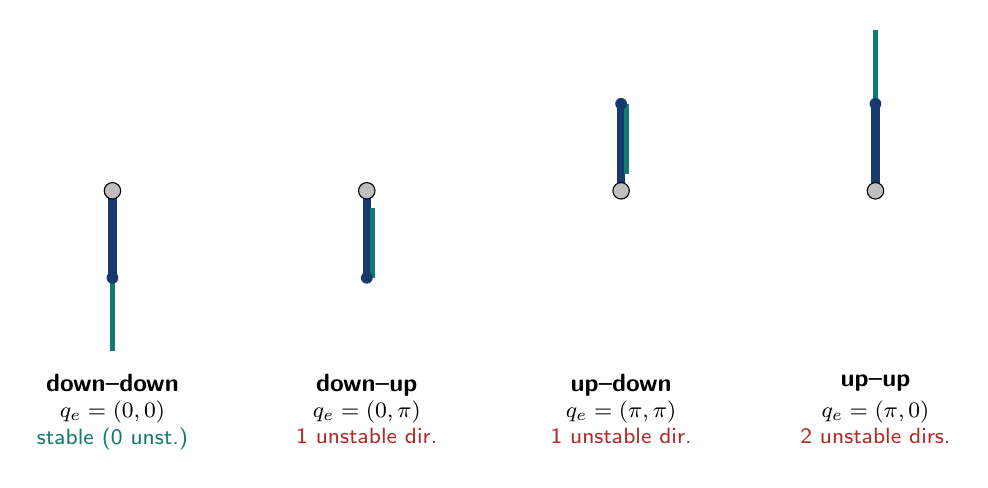
\begin{tikzpicture}[scale=0.85]
  % Down-down (0,0)
  \begin{scope}[shift={(0,0)}]
    \draw[line width=3pt, navy] (0,0) -- (0,-1.3);
    \draw[line width=1.8pt, accentteal] (0,-1.3) -- (0,-2.4);
    \fill[gray!50, draw=black] (0,0) circle (3.5pt);
    \fill[navy] (0,-1.3) circle (2.5pt);
    \node[below, font=\small\bfseries] at (0,-2.6) {down--down};
    \node[below, font=\footnotesize] at (0,-3.0) {$q_e = (0,0)$};
    \node[below, font=\footnotesize, accentteal] at (0,-3.4) {stable (0 unst.)};
  \end{scope}
  % Down-up (0,pi)
  \begin{scope}[shift={(3.8,0)}]
    \draw[line width=3pt, navy] (0,0) -- (0,-1.3);
    \draw[line width=1.8pt, accentteal] (0.08,-1.3) -- (0.08,-0.25);
    \fill[gray!50, draw=black] (0,0) circle (3.5pt);
    \fill[navy] (0,-1.3) circle (2.5pt);
    \node[below, font=\small\bfseries] at (0,-2.6) {down--up};
    \node[below, font=\footnotesize] at (0,-3.0) {$q_e = (0,\pi)$};
    \node[below, font=\footnotesize, accentred] at (0,-3.4) {1 unstable dir.};
  \end{scope}
  % Up-down (pi,pi)
  \begin{scope}[shift={(7.6,0)}]
    \draw[line width=3pt, navy] (0,0) -- (0,1.3);
    \draw[line width=1.8pt, accentteal] (0.08,1.3) -- (0.08,0.25);
    \fill[gray!50, draw=black] (0,0) circle (3.5pt);
    \fill[navy] (0,1.3) circle (2.5pt);
    \node[below, font=\small\bfseries] at (0,-2.6) {up--down};
    \node[below, font=\footnotesize] at (0,-3.0) {$q_e = (\pi,\pi)$};
    \node[below, font=\footnotesize, accentred] at (0,-3.4) {1 unstable dir.};
  \end{scope}
  % Up-up (pi,0)
  \begin{scope}[shift={(11.4,0)}]
    \draw[line width=3pt, navy] (0,0) -- (0,1.3);
    \draw[line width=1.8pt, accentteal] (0,1.3) -- (0,2.4);
    \fill[gray!50, draw=black] (0,0) circle (3.5pt);
    \fill[navy] (0,1.3) circle (2.5pt);
    \node[below, font=\small\bfseries] at (0,-2.6) {up--up};
    \node[below, font=\footnotesize] at (0,-3.0) {$q_e = (\pi,0)$};
    \node[below, font=\footnotesize, accentred] at (0,-3.4) {2 unstable dirs.};
  \end{scope}
\end{tikzpicture}
\caption{The four natural equilibria of the two-link pendulum. Link 2 is drawn thinner and colored so folded configurations remain visible \emph{(slide 50)}.}
\label{fig:four_eq}
\end{figure}

\begin{table}[ht]
\centering
\caption{Natural equilibria and linearized dynamics of the two-link pendulum \emph{(slide 51)}.}
\label{tab:twolink_eq}
\renewcommand{\arraystretch}{1.2}
\begin{tabular}{@{}l l p{8.4cm}@{}}
\toprule
\textbf{Equilibrium} & \textbf{$K_e$} & \textbf{Small motions (reference values)} \\
\midrule
down--down $(0,0)$ & Positive definite & Two oscillations: $5.10\,\mathrm{rad/s}$ (period $1.23\,\mathrm{s}$, in-phase, $\delta q_2/\delta q_1 = 0.69$) and $11.6\,\mathrm{rad/s}$ (period $0.54\,\mathrm{s}$, out-of-phase, $\delta q_2/\delta q_1 = -3.4$). \\
down--up $(0,\pi)$ & 1 negative eig. & Falls at $8.29\,\mathrm{s}^{-1}$; oscillates at $7.13\,\mathrm{rad/s}$. \\
up--down $(\pi,\pi)$ & 1 negative eig. & Falls at $7.13\,\mathrm{s}^{-1}$; oscillates at $8.29\,\mathrm{rad/s}$. \\
up--up $(\pi,0)$ & Negative definite & Falls in two directions: $5.10\,\mathrm{s}^{-1}$ and $11.6\,\mathrm{s}^{-1}$ ($1/\lambda = 0.086\,\mathrm{s}$). \\
\bottomrule
\end{tabular}
\end{table}

\begin{intuition}[Why Balancing Two Inverted Links Is Hard]
The frequencies come in symmetric pairs because flipping both links from $(0,0)$ to $(\pi,0)$ (or $(0,\pi)$ to $(\pi,\pi)$) leaves $M_e$ unchanged and simply negates $K_e$. Crucially, the up--up position falls in $1/11.6 = 0.086\,\mathrm{s}$---more than twice as fast as the single pendulum ($0.20\,\mathrm{s}$). Balancing a double inverted pendulum is intrinsically difficult because of this fast instability, even before counting how many motors it has!
\end{intuition}

\subsection{Held Equilibria, Stability Criterion, and Equilibrium Map (Q3) \emph{(slides 52--54)}}

A constant torque creates one-parameter curves of forced equilibria in configuration space (one passive constraint leaves one free parameter):
\begin{itemize}
  \item \textbf{Pendubot ($G_1 = \tau_e,\; G_2 = 0$):} The passive row requires $\sin(q_1 + q_2) = 0$, so link 2 must be vertical (hanging or standing) while $q_1$ is free:
  \[
    q_1 + q_2 \in \{0, \pi\}, \qquad \tau_e = a \sin q_1.
  \]
  Example: holding $q_1 = 60^\circ$ requires $\tau_e = 2.55\,\mathrm{Nm}$.
  \item \textbf{Acrobot ($G_1 = 0,\; G_2 = \tau_e$):} The passive row requires $x_G = 0$, placing the overall CoM on the vertical line through the shoulder (below or above it) while $q_2$ is free:
  \[
    \tan q_1 = -\frac{b\sin q_2}{a + b\cos q_2}, \qquad \tau_e = b\sin(q_1 + q_2).
  \]
  Example: at $q_2 = 90^\circ$, $q_1 = -14.0^\circ$ and $\tau_e = 0.71\,\mathrm{Nm}$.
\end{itemize}

\begin{proposition}[Stable Held Postures \emph{(slide 53)}]
An equilibrium held by a constant torque---whether at the shoulder (Pendubot) or at the elbow (Acrobot)---is stable if and only if
\[
  \cos q_1 > 0 \quad \text{and} \quad \cos(q_1 + q_2) > 0,
\]
that is, if and only if \emph{both links point below the horizontal}.
\end{proposition}

\begin{proof}
Since $B$ is constant, $\tau_e$ does not enter $K_e$. By Sylvester's criterion (applied from the lower-right corner), the symmetric $2 \times 2$ matrix $K_e$ is positive definite if and only if its $(2,2)$ entry $b\cos(q_1+q_2) > 0$ and its determinant $ab\cos q_1 \cos(q_1+q_2) > 0$, which is equivalent to $\cos q_1 > 0$ and $\cos(q_1+q_2) > 0$.
\end{proof}

Numerically: for the Pendubot, $(60^\circ, -60^\circ)$ (link 2 hanging) is stable and oscillates at $4.29$ and $7.68\,\mathrm{rad/s}$, while $(60^\circ, 120^\circ)$ (link 2 standing) falls at $7.31\,\mathrm{s}^{-1}$. For the Acrobot, the lower branch is stable for $|q_2| < 104.5^\circ$; at $(-14^\circ, 90^\circ)$ it oscillates at $3.45$ and $6.17\,\mathrm{rad/s}$.

\begin{figure}[ht]
\centering
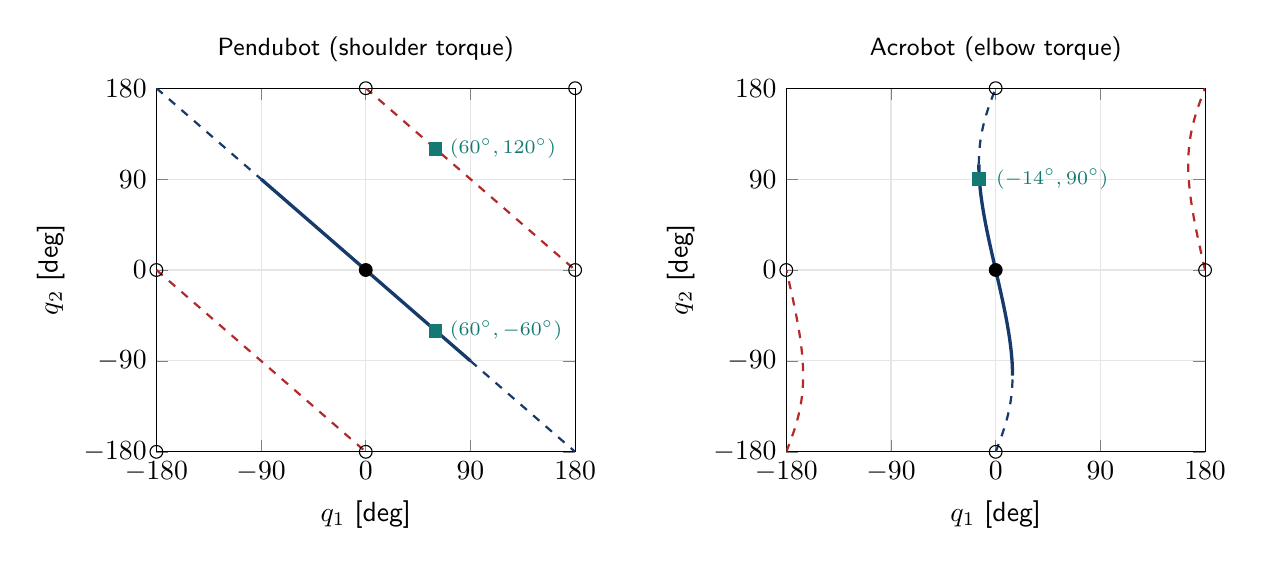
\begin{tikzpicture}
  % Left: Pendubot equilibrium map
  \begin{axis}[
    width=6.9cm, height=6.2cm,
    title={\small Pendubot (shoulder torque)},
    xlabel={$q_1$ [deg]}, ylabel={$q_2$ [deg]},
    xmin=-180, xmax=180, ymin=-180, ymax=180,
    xtick={-180,-90,0,90,180}, ytick={-180,-90,0,90,180},
    grid=major, grid style={gray!20}
  ]
    % q1 + q2 = 0 (stable for |q1| < 90)
    \addplot[very thick, navy, domain=-90:90] {-x};
    \addplot[thick, navy, dashed, domain=-180:-90] {-x};
    \addplot[thick, navy, dashed, domain=90:180] {-x};
    % q1 + q2 = 180 and -180 (unstable: cos(q1+q2) = -1)
    \addplot[thick, accentred, dashed, domain=0:180] {180 - x};
    \addplot[thick, accentred, dashed, domain=-180:0] {-180 - x};
    % Natural equilibria
    \addplot[only marks, mark=*, black, mark size=2.3pt] coordinates {(0,0)};
    \addplot[only marks, mark=o, black, mark size=2.3pt] coordinates {(0,180) (0,-180) (180,180) (-180,-180) (180,0) (-180,0)};
    % Examples
    \addplot[only marks, mark=square*, accentteal, mark size=2.3pt] coordinates {(60,-60) (60,120)};
    \node[font=\scriptsize, right, accentteal] at (axis cs:64,-60) {$(60^\circ,-60^\circ)$};
    \node[font=\scriptsize, right, accentteal] at (axis cs:64,120) {$(60^\circ,120^\circ)$};
  \end{axis}

  % Right: Acrobot equilibrium map
  \begin{axis}[
    xshift=8.0cm,
    width=6.9cm, height=6.2cm,
    title={\small Acrobot (elbow torque)},
    xlabel={$q_1$ [deg]}, ylabel={$q_2$ [deg]},
    xmin=-180, xmax=180, ymin=-180, ymax=180,
    xtick={-180,-90,0,90,180}, ytick={-180,-90,0,90,180},
    grid=major, grid style={gray!20},
    samples=100
  ]
    % Lower CoM branch: q1 = atan(-0.736 sin(q2) / (2.943 + 0.736 cos(q2)))
    % Solid for |q2| < 104.5, dashed outside
    \addplot[very thick, navy, domain=-104.5:104.5] ({atan(-0.736*sin(x)/(2.943+0.736*cos(x)))}, {x});
    \addplot[thick, navy, dashed, domain=104.5:180] ({atan(-0.736*sin(x)/(2.943+0.736*cos(x)))}, {x});
    \addplot[thick, navy, dashed, domain=-180:-104.5] ({atan(-0.736*sin(x)/(2.943+0.736*cos(x)))}, {x});
    % Upper CoM branch (shifted by +-180 deg, wrapped into [-180, 180])
    \addplot[thick, accentred, dashed, domain=-180:0] ({atan(-0.736*sin(x)/(2.943+0.736*cos(x))) - 180}, {x});
    \addplot[thick, accentred, dashed, domain=0:180] ({atan(-0.736*sin(x)/(2.943+0.736*cos(x))) + 180}, {x});
    % Natural equilibria
    \addplot[only marks, mark=*, black, mark size=2.3pt] coordinates {(0,0)};
    \addplot[only marks, mark=o, black, mark size=2.3pt] coordinates {(0,180) (0,-180) (180,0) (-180,0)};
    % Example
    \addplot[only marks, mark=square*, accentteal, mark size=2.3pt] coordinates {(-14,90)};
    \node[font=\scriptsize, right, accentteal] at (axis cs:-8,90) {$(-14^\circ,90^\circ)$};
  \end{axis}
\end{tikzpicture}
\caption{Map of constant-torque equilibria in $(q_1, q_2)$ space (opposite edges identified). Solid: stable; dashed: unstable; black dot/circles: natural equilibria; squares: worked examples \emph{(slide 54)}.}
\label{fig:eq_map}
\end{figure}

\subsection{Linear Models at Top/Bottom and Inertial Coupling (Q5) \emph{(slides 55--57)}}

At $(0,0)$ and $(\pi,0)$ the arm is straight, so $M_e$ is identical and $K_e$ differs only in sign:
\[
  M_e = \begin{bmatrix} 0.135 & 0.0375 \\ 0.0375 & 0.015 \end{bmatrix}, \qquad
  K_e = \pm \begin{bmatrix} 3.679 & 0.736 \\ 0.736 & 0.736 \end{bmatrix} \quad (+ \text{ bottom},\; - \text{ top}).
\]
Solving for accelerations at the upright equilibrium $(\pi, 0)$ yields
\[
  \delta\ddot{q} = \begin{bmatrix} 44.6 & -26.8 \\ -62.4 & 115.9 \end{bmatrix} \delta q + b\,\delta\tau,
  \qquad b_P = \begin{bmatrix} 24.2 \\ -60.6 \end{bmatrix}, \quad b_A = \begin{bmatrix} -60.6 \\ 218.2 \end{bmatrix}.
\]
Both entries of $b = M_e^{-1} B$ are nonzero: a single motor accelerates \emph{both} joints at once in opposite directions.

\textbf{Q5 (Inertial Coupling):} The motor reaches the passive joint through $M_{12}(q_2) = I_2 + m_2 \ell_{c2}^2 + m_2 \ell_1 \ell_{c2}\cos q_2$. For our reference arm, $M_{12}(q_2) = 0.015 + 0.0225\cos q_2$, which is $0.0375$ when straight, \emph{vanishes} at $q_2 = \pm 131.8^\circ$, and becomes negative ($-0.0075$) when folded (Figure~\ref{fig:coupling}). For the Pendubot starting from rest (ignoring gravity), $\ddot{q}_2 = -(M_{12}/M_{22})\ddot{q}_1$: $-2.5\ddot{q}_1$ straight (link 2 left behind), $0$ at $\pm 131.8^\circ$, and $+0.5\ddot{q}_1$ folded. The coupling never vanishes if $I_2 + m_2 \ell_{c2}^2 > m_2 \ell_1 \ell_{c2}$ (e.g., with a short first link).

\begin{figure}[ht]
\centering
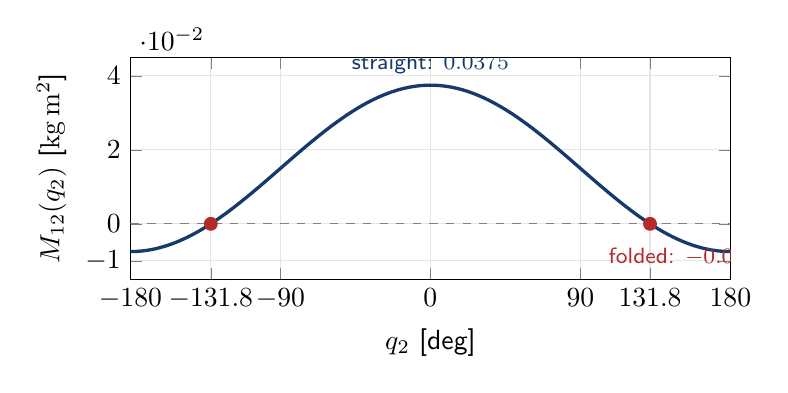
\begin{tikzpicture}
  \begin{axis}[
    width=9.2cm, height=4.4cm,
    xlabel={$q_2$ [deg]}, ylabel={$M_{12}(q_2)$ [$\mathrm{kg\,m^2}$]},
    xmin=-180, xmax=180, ymin=-0.015, ymax=0.045,
    xtick={-180,-131.8,-90,0,90,131.8,180},
    xticklabels={$-180$,$-131.8$,$-90$,$0$,$90$,$131.8$,$180$},
    ytick={-0.01, 0, 0.02, 0.04},
    grid=major, grid style={gray!20},
    samples=100
  ]
    \addplot[very thick, navy, domain=-180:180] {0.015 + 0.0225*cos(x)};
    \addplot[dashed, gray, domain=-180:180] {0};
    \addplot[only marks, mark=*, accentred, mark size=2.3pt] coordinates {(-131.8, 0) (131.8, 0)};
    \node[font=\footnotesize, above, navy] at (axis cs:0,0.038) {straight: $0.0375$};
    \node[font=\footnotesize, above, accentred] at (axis cs:155,-0.014) {folded: $-0.0075$};
  \end{axis}
\end{tikzpicture}
\caption{Inertial coupling $M_{12}(q_2) = 0.015 + 0.0225\cos q_2$ of the reference two-link pendulum, vanishing and changing sign at $q_2 = \pm 131.8^\circ$ \emph{(slide 56)}.}
\label{fig:coupling}
\end{figure}

% ============================================================================
\section{Part 5: Reaction Wheel, Planar VTOL, and the Input Matrix \emph{(slides 58--66)}}
% ============================================================================

\subsection{The Reaction-Wheel Pendulum \emph{(slides 59--62)}}

A pendulum body (angle $q_1$ from downward vertical, upright at $q_1 = \pi$) carries a balanced flywheel (relative angle $q_2$) driven by an internal motor torque $\tau$. Let $I_b$ be the inertia of body and wheel about the pivot (without wheel spin), $I_w$ the axial inertia of the wheel, and $\kappa = m_{\text{tot}} g d$. This is simply the two-link pendulum with $\ell_{c2} = 0$ and $I_2 = I_w$:
\[
  T = \frac{1}{2} I_b \dot{q}_1^2 + \frac{1}{2} I_w (\dot{q}_1 + \dot{q}_2)^2, \qquad
  V = -\kappa \cos q_1, \qquad \delta W = \tau \delta q_2,
\]
leading to the linear-inertia dynamic model (with $h \equiv 0$):
\begin{equation}
  \begin{bmatrix} I_b + I_w & I_w \\ I_w & I_w \end{bmatrix}
  \begin{bmatrix} \ddot{q}_1 \\ \ddot{q}_2 \end{bmatrix}
  + \begin{bmatrix} \kappa \sin q_1 \\ 0 \end{bmatrix}
  = \begin{bmatrix} 0 \\ \tau \end{bmatrix}
  \quad\Longleftrightarrow\quad
  I_b \ddot{q}_1 + \kappa \sin q_1 = -\tau, \quad I_w(\ddot{q}_1 + \ddot{q}_2) = \tau.
  \label{eq:rwp}
\end{equation}

\begin{figure}[ht]
\centering
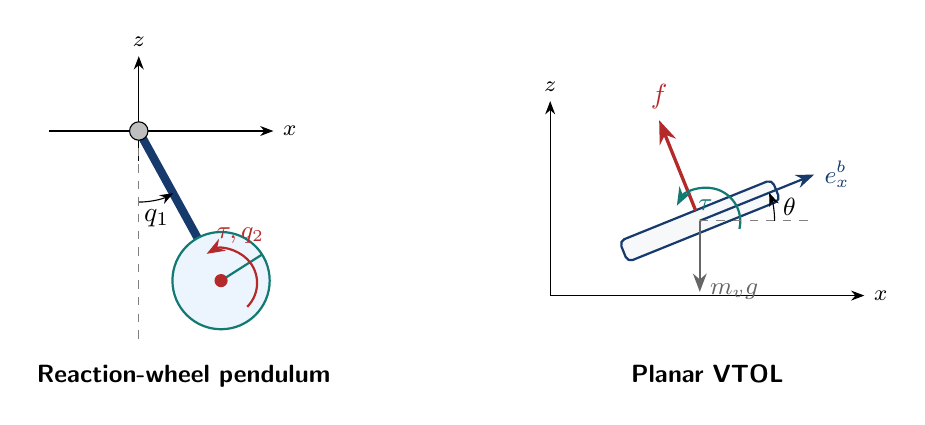
\begin{tikzpicture}[scale=0.95, >=Stealth]
  % Left: Reaction-wheel pendulum
  \begin{scope}[shift={(0,0)}]
    \draw[->] (-1.2,0) -- (1.8,0) node[right, font=\footnotesize] {$x$};
    \draw[->] (0,-0.4) -- (0,1.0) node[above, font=\footnotesize] {$z$};
    \draw[dashed, gray] (0,0) -- (0,-2.8);
    % Pendulum arm
    \draw[line width=3pt, navy] (0,0) -- (1.1,-2.0);
    \fill[gray!50, draw=black] (0,0) circle (3.5pt);
    % Wheel
    \draw[thick, fill=intuitionbg, draw=accentteal] (1.1,-2.0) circle (0.65);
    \draw[thick, accentteal] (1.1,-2.0) -- (1.65,-1.65);
    \fill[accentred] (1.1,-2.0) circle (2.5pt);
    % Angles & torque
    \draw[->] (0,-0.95) arc (-90:-61:0.95) node[midway, below] {$q_1$};
    \draw[->, thick, accentred] (1.45,-2.35) arc (-45:120:0.45) node[above right, font=\small] {$\tau, q_2$};
    \node[below, font=\small\bfseries] at (0.6,-3.0) {Reaction-wheel pendulum};
  \end{scope}

  % Right: Planar VTOL
  \begin{scope}[shift={(7.5,-1.2)}]
    \draw[->] (-2.0,-1.0) -- (2.2,-1.0) node[right, font=\footnotesize] {$x$};
    \draw[->] (-2.0,-1.0) -- (-2.0,1.6) node[above, font=\footnotesize] {$z$};
    % Body tilted by theta = 22 deg
    \begin{scope}[rotate=22]
      \draw[thick, fill=thmbg, draw=navy, rounded corners=2pt] (-1.1,-0.15) rectangle (1.1,0.15);
      \draw[->, very thick, accentred] (0,0.15) -- (0,1.45) node[above] {$f$};
      \draw[->, thick, navy] (0,0) -- (1.65,0) node[right, font=\small] {$e_x^b$};
      \draw[->, thick, accentteal] (0.45,-0.3) arc (-35:130:0.45) node[right, xshift=4pt, font=\small] {$\tau$};
    \end{scope}
    \draw[dashed, gray] (0,0) -- (1.5,0);
    \draw[->] (1.0,0) arc (0:22:1.0) node[midway, right, font=\small] {$\theta$};
    \draw[->, thick, gray!80!black] (0,0) -- (0,-0.95) node[right, font=\small] {$m_v g$};
    \node[below, font=\small\bfseries] at (0.1,-1.8) {Planar VTOL};
  \end{scope}
\end{tikzpicture}
\caption{Schematics of the reaction-wheel pendulum (left) and the planar VTOL (right) \emph{(slides 59, 63)}.}
\label{fig:rwp_vtol}
\end{figure}

\begin{itemize}
  \item \textbf{Q1, Q2, Q5 (Structure, Momentum, Coupling):} $M$ is constant, $h = 0$, and the coupling $M_{12} = I_w$ never vanishes or changes sign. Both rows are angular momentum balances: $p_2 = I_w(\dot{q}_1+\dot{q}_2)$ obeys $\dot{p}_2 = \tau$ (wheel spin changed only by motor), and $p_1 = (I_b+I_w)\dot{q}_1 + I_w\dot{q}_2$ obeys $\dot{p}_1 = -\kappa\sin q_1$ (total momentum changed only by gravity). With motor off ($\tau=0$), $p_2$ is conserved and the body swings with inertia $I_b$ ($\omega = 6.12\,\mathrm{rad/s}$ vs.\ $6.05\,\mathrm{rad/s}$ with the wheel locked). Without gravity, $p_1$ is conserved; from rest, $(I_b+I_w)q_1 + I_w q_2 = \text{const}$, so turning the body by $10^\circ$ requires spinning the wheel by $-410^\circ$.
  \item \textbf{Q3 (An Impossible Posture):} $G = (\kappa\sin q_1, 0)^T$ and $B = (0,1)^T$ force $\sin q_1 = 0$, $\tau_e = 0$ ($q_2$ arbitrary). Why can't $\tau = -\kappa\sin\bar{q}_1$ hold a tilted posture $\bar{q}_1$? It balances gravity on the body, \emph{but the same reaction torque accelerates the wheel without bound!} A steady motion exists with the body vertical and the wheel spinning at constant speed (since $q_2$ is cyclic and often dropped from the state).
  \item \textbf{Q4 (Small Motions):} Upright, the body falls at $\lambda = \sqrt{\kappa/I_b} = 6.12\,\mathrm{s}^{-1}$, while $q_2$ drifts:
  \[
    \delta\ddot{q}_1 = 37.5\,\delta q_1 - 25\,\delta\tau, \qquad
    \delta\ddot{q}_2 = -37.5\,\delta q_1 + 1025\,\delta\tau.
  \]
\end{itemize}

\begin{intuition}[The Angular Momentum Budget]
The wheel accelerates $40\times$ more than the body in the opposite direction ($1025$ vs.\ $-25$). Because the motor merely exchanges angular momentum between wheel and body without creating any, the wheel speed acts as a finite \emph{budget}: every balancing correction spends wheel speed, so a practical controller must also regulate the wheel speed back to zero.
\end{intuition}

\subsection{The Planar VTOL: A Body-Fixed Force \emph{(slides 63--65)}}

A planar vertical take-off and landing (VTOL) vehicle has coordinates $q = (x, z, \theta)^T$ and inputs $u = (f, \tau)^T$ (thrust $f$ along the body vertical axis, pitching moment $\tau$). Its energies are $T = \frac{1}{2} m_v (\dot{x}^2 + \dot{z}^2) + \frac{1}{2} I \dot{\theta}^2$ and $V = m_v g z$. Virtual work gives $\delta W = -f\sin\theta\,\delta x + f\cos\theta\,\delta z + \tau\,\delta\theta$, so
\begin{equation}
  \begin{bmatrix} m_v & 0 & 0 \\ 0 & m_v & 0 \\ 0 & 0 & I \end{bmatrix} \ddot{q}
  + \begin{bmatrix} 0 \\ m_v g \\ 0 \end{bmatrix}
  = B(\theta) \begin{bmatrix} f \\ \tau \end{bmatrix}, \qquad
  B(\theta) = \begin{bmatrix} -\sin\theta & 0 \\ \cos\theta & 0 \\ 0 & 1 \end{bmatrix}.
  \label{eq:vtol}
\end{equation}
\begin{itemize}
  \item \textbf{Q1 (Structure):} $M$ is constant and diagonal ($h = 0$, zero inertial coupling); all nonlinearity lives in $B(\theta)$ of rank $2 < 3$. Choosing the left annihilator $N(\theta)^T = (\cos\theta, \sin\theta, 0)$ (so $N^T B = 0$) yields the single passive equation:
  \[
    m_v \cos\theta\,\ddot{x} + m_v \sin\theta\,\ddot{z} + m_v g \sin\theta = 0,
  \]
  which is Newton's law along the body horizontal axis $e_x^b$: there is no actuator force perpendicular to the thrust.
  \item \textbf{Q2 (Energy):} $\dot{E} = f(-\sin\theta\,\dot{x} + \cos\theta\,\dot{z}) + \tau\dot{\theta}$; thrust does work only along its own direction.
  \item \textbf{Q5 (Coupling):} Rather than inertial coupling, the VTOL uses \emph{configuration coupling}: $\tau \to \theta \to \text{direction of } f \to x$.
  \item \textbf{Q3 (Hover and Tilt):} $G = B(\theta_e)u_e$ with $f_e \ge 0$ gives level hover: $\theta_e = 0$, $f_e = m_v g$, $\tau_e = 0$, at any $(x_e, z_e)$. Maintaining a constant tilt $\bar{\theta}$ at constant altitude ($\ddot{z}=0$) produces lateral acceleration $\ddot{x} = -g\tan\bar{\theta}$.
  \item \textbf{Q4 (Small Motions):} Because $B(\theta)$ depends on $\theta$, $K_e = \partial(G - B u_e)/\partial q$ is \emph{not symmetric}. Linearizing around hover gives
  \[
    \delta\ddot{x} = -g\delta\theta, \qquad \delta\ddot{z} = \frac{\delta f}{m_v}, \qquad \delta\ddot{\theta} = \frac{\delta\tau}{I}
    \quad\Longrightarrow\quad
    \frac{d^4}{dt^4}\delta x = -\frac{g}{I}\delta\tau.
  \]
  All characteristic values are zero: a disturbed hover drifts, and lateral position is reached through a chain of four integrators.
\end{itemize}

\begin{intuition}[Two Ways of Being Underactuated]
Pendulum-type systems have a coordinate without a motor, reached through \emph{inertial coupling} ($M_{12}$). The planar VTOL has no inertial coupling: every coordinate can be pushed, but the push has a fixed direction in the body and must be aimed by rotating it. In both cases, some linear combination of the equations of motion contains no input.
\end{intuition}

\subsection{The Input Matrix in General \emph{(slide 66)}}

\begin{definition}[Generic Actuation Rank and Passive Equations]
The number of independent inputs is $p = \max_q \operatorname{rank} B(q)$. If $p < m$, there exists a full-rank matrix $N(q) \in \mathbb{R}^{m \times (m-p)}$ satisfying $N(q)^T B(q) = 0$, yielding $m - p$ \textbf{passive equations} (second-order nonholonomic constraints that every feasible trajectory must obey):
\[
  N(q)^T \big(M(q)\ddot{q} + h(q,\dot{q}) + G(q)\big) = 0.
\]
\end{definition}

Under a smooth coordinate change $q = f(z)$ with Jacobian $J = \partial f/\partial z$, the input matrix transforms as $B_z = J^T B_q$; its entries change (e.g., Acrobot in absolute angles has $B = (-1,1)^T$), but its rank is invariant. A constant $B$ can always be transformed into zeros and ones by a linear change of coordinates, whereas for configuration-dependent $B(q)$ finding coordinates in which $B_z$ is constant requires an integrability condition. Finally, a drop in $\operatorname{rank} B(q)$ at isolated configurations (such as a stretched arm or a lever at dead center) is an \textbf{actuation singularity} of a fully actuated robot, not underactuation.

% ============================================================================
\section{Summary and Model Comparison Sheet}
% ============================================================================

Table~\ref{tab:summary_sheet} consolidates all five systems across the five structural questions, and Figure~\ref{fig:fall_rates} compares the upright instability rates $\lambda$ across the inverted benchmark models using the lecture's reference parameters.

\begin{table}[ht]
\centering
\caption{Master comparison sheet of the five dynamic models across Q1--Q5.}
\label{tab:summary_sheet}
\footnotesize
\renewcommand{\arraystretch}{1.25}
\begin{tabular}{@{}p{2.2cm} c p{2.7cm} p{2.5cm} p{2.5cm} p{2.3cm} p{2.4cm}@{}}
\toprule
\textbf{System} & $(m,p)$ & \textbf{Q1: Passive eq.} & \textbf{Q2: Conserved} & \textbf{Q3: Equilibria} & \textbf{Q4: Upright $\lambda$} & \textbf{Q5: Coupling} \\
\midrule
\textbf{Pendulum} & $(1,1)$ or $(1,0)$ & None (or whole eq.\ if $\tau=0$) & $E$ if $\tau=0$ & $\sin\theta_e = \tau_e/(m_p g \ell_c)$ & $4.95\,\mathrm{s}^{-1}$ ($0.20\,\mathrm{s}$) & Vacuous \\
\textbf{Cart--pendulum} & $(2,1)$ & $\ddot{\theta} = \frac{1}{\ell_{\text{eq}}}(g\sin\theta - \ddot{x}\cos\theta)$ & $p_x$ ($x$ cyclic) if $F=0$ & $\theta_e \in \{0,\pi\}$, $x_e$ free, $F_e=0$ & $5.29\,\mathrm{s}^{-1}$ ($0.19\,\mathrm{s}$); RHP zero $+\omega_0$ & $M_{12} = m_p \ell_c \cos\theta$; zero at $\pm 90^\circ$ \\
\textbf{Pendubot} & $(2,1)$ & Link 2 about elbow ($G_2=0$ at rest) & None with $g$; none even if $g=0$ & $q_1+q_2\in\{0,\pi\}$, $\tau_e=a\sin q_1$ & $5.10$ \& $11.6\,\mathrm{s}^{-1}$ ($0.086\,\mathrm{s}$) & $M_{12}(q_2)$; zero at $\pm 131.8^\circ$ \\
\textbf{Acrobot} & $(2,1)$ & Total arm about shoulder ($x_G=0$ at rest) & $p_1$ if $g=0$ (even with $\tau$) & $x_G = 0$, $\tau_e = b\sin(q_1+q_2)$ & $5.10$ \& $11.6\,\mathrm{s}^{-1}$ ($0.086\,\mathrm{s}$) & $M_{12}(q_2)$; zero at $\pm 131.8^\circ$ \\
\textbf{Reaction wheel} & $(2,1)$ & Total momentum $\dot{p}_1 = -\kappa\sin q_1$ & $p_2$ if $\tau=0$; $p_1$ if $g=0$ & $q_1\in\{0,\pi\}$, $q_2$ free, $\tau_e=0$ & $6.12\,\mathrm{s}^{-1}$ ($0.16\,\mathrm{s}$); $q_2$ drifts & Constant $M_{12} = I_w \neq 0$ \\
\textbf{Planar VTOL} & $(3,2)$ & Force along $e_x^b$ is zero ($N^T B = 0$) & $E$ if $u=0$ & Level hover $\theta_e=0$, $f_e=m_v g$ & All $\mu_i=0$ (drift; $d^4\delta x/dt^4 \propto \delta\tau$) & Config.\ coupling via $B(\theta)$ \\
\bottomrule
\end{tabular}
\end{table}

\begin{figure}[ht]
\centering
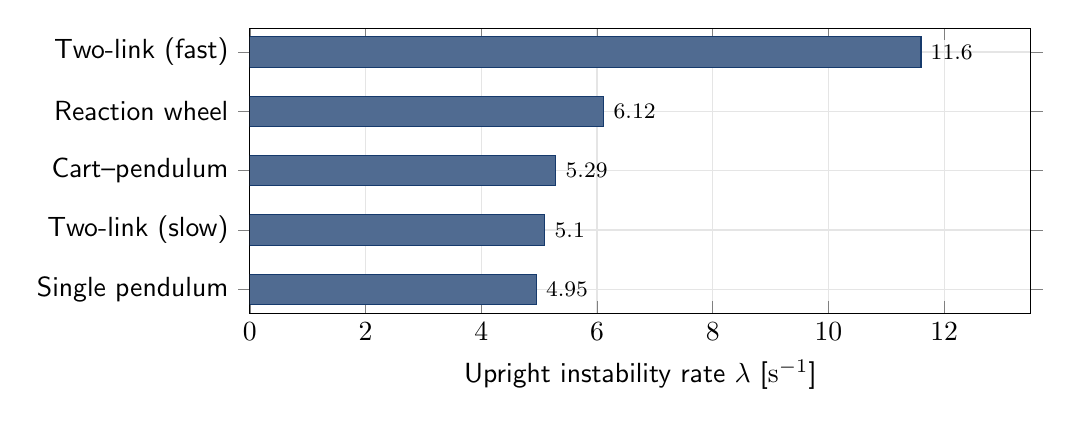
\begin{tikzpicture}
  \begin{axis}[
    xbar,
    width=11.5cm, height=5.2cm,
    xlabel={Upright instability rate $\lambda$ [$\mathrm{s}^{-1}$]},
    xmin=0, xmax=13.5,
    symbolic y coords={{Single pendulum}, {Two-link (slow)}, {Cart--pendulum}, {Reaction wheel}, {Two-link (fast)}},
    ytick=data,
    nodes near coords,
    nodes near coords align={horizontal},
    bar width=11pt,
    grid=major, grid style={gray!20},
    every node near coord/.append style={font=\footnotesize}
  ]
    \addplot[fill=navy!75, draw=navy] coordinates {
      (4.95,{Single pendulum})
      (5.10,{Two-link (slow)})
      (5.29,{Cart--pendulum})
      (6.12,{Reaction wheel})
      (11.6,{Two-link (fast)})
    };
  \end{axis}
\end{tikzpicture}
\caption{Comparison of upright exponential fall rates $\lambda$ across the inverted benchmark models (reference parameters). Higher $\lambda$ means a shorter reaction window $1/\lambda$.}
\label{fig:fall_rates}
\end{figure}

\subsection*{Key Take-Aways}
\begin{itemize}
  \item \textbf{Structure over numbers:} Deriving small models by hand exposes the passive equations ($N^T B = 0$), cyclic coordinates, and coupling zeros that govern controllability, integrability, and control design.
  \item \textbf{Potential energy sets stability; inertia sets speed:} For constant $B$, $K_e = \partial^2 V / \partial q^2$ alone determines whether an equilibrium is stable (and constant inputs do not alter $K_e$), while $M_e$ sets oscillation frequencies and fall rates.
  \item \textbf{Passive equations restrict equilibria and enforce recoil:} Underactuated systems cannot rest at arbitrary postures; free motion along cyclic coordinates causes recoil (cart--pendulum) or consumes a finite momentum budget (reaction wheel).
  \item \textbf{Two mechanisms of underactuation:} Inputs reach unactuated directions either through off-diagonal inertial coupling $M_{ij}(q)$ (which can vanish and change sign, as at $\theta = \pm 90^\circ$ or $q_2 = \pm 131.8^\circ$) or through configuration-dependent input directions $B(q)$ (planar VTOL).
  \item \textbf{Motor placement matters even on identical mechanics:} The Acrobot and Pendubot share the exact same $M, h, G$, yet swapping $B$ changes momentum conservation, equilibrium manifolds, and how the single torque distributes acceleration across the joints.
\end{itemize}

\end{document}